%==============================================================================
% PLDP: Patient-Level Differential Privacy in Hierarchical Federated Learning
% for Multimodal Medical IoT. IEEE journal manuscript (IEEEtran, journal).
%
% Compile with pdfLaTeX: pdflatex -> bibtex -> pdflatex -> pdflatex
% (Overleaf does this automatically; main document: main.tex).
%==============================================================================
\documentclass[journal]{IEEEtran}

\usepackage[T1]{fontenc}
\usepackage[utf8]{inputenc}
\usepackage{cite}
\usepackage{amsmath,amssymb}
\usepackage{graphicx}
\graphicspath{{figures/}}
\usepackage{booktabs}
\usepackage{array}
\usepackage{multirow}
\usepackage{algorithm}
\usepackage{algorithmic}
\usepackage{stfloats}
\usepackage{xcolor}
\usepackage{url}
\usepackage[hidelinks]{hyperref}

\newtheorem{theorem}{Theorem}
\newtheorem{corollary}{Corollary}
\newtheorem{proposition}{Proposition}
\newcommand{\pend}[1]{#1}
% Explanatory note set under a table, so captions stay to two lines.
\newcommand{\tabnote}[1]{\par\vspace{3pt}\parbox{\linewidth}{\footnotesize #1}}

\begin{document}

\title{Patient-Level Differential Privacy in Hierarchical\\
       Federated Learning for Multimodal Medical IoT}

% (College grid) Authors as a grid under the title. Three columns of long e-mail addresses
% are wider than the page at the default author size; \small and tighter
% columns make the row fit.
% Author block: two layouts of the same authors.
%   \collegeauthorstrue  -> grid under the title (college format; default)
%   \collegeauthorsfalse -> IEEE journal format: names on one line, affiliation
%                           and e-mail in the first-page \thanks footnote, as the
%                           IEEE double-column journal template requires
%                           (IoT-J). ORCID iDs are entered in the submission portal.
\newif\ifcollegeauthors
\collegeauthorsfalse   % IoT-J submission: IEEE journal author format
\ifcollegeauthors
\author{
{\small\setlength{\tabcolsep}{2pt}%
\begin{tabular}{ccc}
\begin{tabular}{c}
Samartha H V\\
\textit{Manipal Institute of Technology Bengaluru}\\
\textit{Manipal Academy of Higher Education}\\
Manipal, India\\
samartha1.mitblr2025@learner.manipal.edu
\end{tabular}
&
\begin{tabular}{c}
Shreyas J\\
\textit{Manipal Institute of Technology Bengaluru}\\
\textit{Manipal Academy of Higher Education}\\
Manipal, India\\
shreyas.j@manipal.edu
\end{tabular}
&
\begin{tabular}{c}
Udayaprasad P K\\
\textit{Manipal Institute of Technology Bengaluru}\\
\textit{Manipal Academy of Higher Education}\\
Manipal, India\\
udayaprasad.mitblr2024@learner.manipal.edu
\end{tabular}
\\ \noalign{\vspace{2.4em}}  % \\[len] is absorbed by the tall cells
\multicolumn{3}{c}{
\begin{tabular}{cc}
\begin{tabular}{c}
Shreelakshmi Yadav N\\
\textit{Manipal Institute of Technology Bengaluru}\\
\textit{Manipal Academy of Higher Education}\\
Manipal, India\\
shreelakshmi.mitblr2024@learner.manipal.edu
\end{tabular}
&
\begin{tabular}{c}
Sowmya T Rao\\
\textit{Manipal Institute of Technology Bengaluru}\\
\textit{Manipal Academy of Higher Education}\\
Manipal, India\\
sowmya.mitblr2024@learner.manipal.edu
\end{tabular}
\end{tabular}
}
\end{tabular}}\vspace{-2.6em}  % less space before the abstract
}
\else
\author{Samartha~H~V, Shreyas~J, Udayaprasad~P~K, Shreelakshmi~Yadav~N,
and Sowmya~T~Rao%
\thanks{\raggedright The authors are with the Manipal Institute of Technology Bengaluru,
Manipal Academy of Higher Education, Manipal, India (e-mail:
samartha1.mitblr2025@learner.manipal.edu; shreyas.j@manipal.edu;
udayaprasad.mitblr2024@learner.manipal.edu;
shreelakshmi.mitblr2024@learner.manipal.edu;
sowmya.mitblr2024@learner.manipal.edu).}}
\fi

% Set the running head once the venue is fixed. Both lines together, or neither.
%\markboth{IEEE Journal Name,~Vol.~XX, No.~XX, Month~2026}%
%{H.~V \MakeLowercase{\textit{et al.}}: Patient-Level Differential Privacy in Hierarchical FL for Medical IoT}

\maketitle

\begin{abstract}
Hierarchical federated learning keeps Internet-of-Things data local, but its
differential-privacy guarantee protects single records, whereas clinical
deployments must protect patients with many records. This paper proposes
a client--edge--cloud framework whose privacy unit is the patient. Each client
clips a patient's summed gradient, calibrates noise to its population and
accounts for every hierarchical release. The guarantee is proved for the training
transcript and, with public encoders and standardization constants, end to
end (eICU). It is evaluated on VitalDB, $187$
eICU hospitals and, at record level, a wearable corpus. At a
training budget of at most $\varepsilon = 0.9$ ($1.0$ including the
conformal release; $0.766$ at record level on WEAR), it reduces uplink traffic
by $90.8$--$96.1\,\%$ and modeled energy per round by $72.3$--$79.6\,\%$;
$95$th-percentile workstation-CPU inference latency is at most $2.3$~ms.
On person-partitioned VitalDB the guarantee costs no utility (area under the
receiver operating characteristic curve, AUC, $0.832$ vs.\ $0.820$
non-private). On eICU it costs $3.1$ points (inconclusive against the
two-point target) and $3.9$ end to end, missing it; a non-private
hierarchical baseline is more accurate ($0.825$ vs.\ $0.794$). It uploads $2.2$--$4.0$ times less than re-implemented hierarchical and private
baselines and leaks less in the VitalDB audit. On VitalDB and WEAR,
pretrained initialization, not head-only noise, makes a strict budget
survivable; the patient-unit cost follows $A(1 - 1/k)$ in records per patient
$k$. A membership-inference audit with a positive control finds record-level
training above its difficulty floor (attack AUC $0.576$) and patient-level
training at it ($0.503$).
\end{abstract}


\begin{IEEEkeywords}
Hierarchical federated learning, Internet of Things, differential privacy,
user-level privacy, membership inference, multimodal learning, edge
computing, clinical decision support.
\end{IEEEkeywords}

\IEEEpeerreviewmaketitle

\section{Introduction}
\label{sec:intro}

\IEEEPARstart{T}{he} Internet of Things (IoT) is increasingly used to monitor
people continuously: in the operating room, in the intensive care unit and
through wearable sensors. Much of the value of these deployments comes from
combining different kinds of data. In an operating room, monitors record
physiological waveforms while the hospital record holds the patient's
clinical history; in a wearable installation, inertial sensors record motion
while a camera records what the wearer sees. A model that sees both streams
can recognize states that neither reveals alone.

Such data cannot simply be collected in one place. Clinical records are
governed by consent and by data-protection law, and continuous multimodal
sensing produces volumes that are costly to move. Federated learning (FL)
\cite{ref1} addresses this by training a shared model where the data reside
and exchanging only model updates. Hierarchical FL \cite{ref2, ref3} adds an
edge tier between the clients and the cloud, so that most aggregation happens
close to the data and the wide-area link is used only once every several
rounds, which reduces both traffic and energy.

Keeping the data local, however, does not by itself keep it private. Model
updates are computed from the records, and an adversary can often infer from
a released model whether a particular record was used in training
\cite{ref14}. Differential privacy (DP) gives a formal guarantee against such
inference. Its standard training algorithm, differentially private stochastic
gradient descent (DP-SGD) \cite{ref6}, bounds (clips) the influence of each
training record and adds calibrated noise, so the guarantee protects whatever
unit is clipped. In a sensing deployment that unit is a short window of
signal, not a person, and every patient contributes many windows. A
record-level guarantee therefore answers whether a particular window was used,
whereas a clinical deployment must answer whether a particular
\emph{patient} was. Group privacy \cite{ref8} relates the two, but at the
group sizes found in our data it turns a nominal $\varepsilon = 1$ into
$\varepsilon \approx 8$ with $\delta \approx 0.09$, which supports no clinical
claim.

Existing work has addressed communication efficiency, privacy and multimodal
learning largely separately. The review in Section~\ref{sec:related}
identifies four gaps.
\begin{enumerate}
\item \emph{No patient-level guarantee across a hierarchy.} Hierarchical
designs \cite{ref3, ref4, ref5} reduce communication and energy but provide no
formal guarantee, and private designs \cite{ref9, ref10} provide one but do
not account for how an edge tier changes each client's privacy expenditure.
Recent systems join a hierarchy with privacy \cite{ref34, ref37} or privacy
with multimodal clinical data \cite{ref35, ref36}; to our knowledge, none
states its guarantee over an individual whose records are grouped before
clipping.
\item \emph{An unmeasured cost.} The utility cost of protecting individuals
rather than records has not been measured on multimodal data paired at the
source, nor related to the number of records each individual contributes.
\item \emph{An implicit condition.} Private training of a small head on frozen
pretrained features \cite{ref12, ref13} is valid end to end only if the
features were pretrained on a population disjoint from the protected one.
This condition is usually left implicit, and it is not known whether the
benefit comes from the pretraining or from privatizing fewer parameters.
\item \emph{Audits at the wrong unit.} Guarantees are usually reported from
mechanism parameters alone and, where audited, audited per record, which is
exactly what a record-level guarantee already protects.
\end{enumerate}

This paper proposes PP-HFM (Patient-Private Hierarchical Federated Multimodal
learning), a client--edge--cloud framework in which the privacy unit is the
patient by construction. Each client sums the gradients of a patient's records
before clipping, so that the patient as a whole has bounded influence, and
calibrates its noise to its own patient population. The main contributions
are as follows.
\begin{itemize}
\item \emph{Patient-level privacy with complete accounting (gap 1).} A
patient-level private training procedure for hierarchical multimodal FL, with
per-client noise calibration, a proof of its guarantee
(Theorem~\ref{thm:guarantee}), and a ledger of every release, edge tier
included, that states which configurations are covered end to end.
\item \emph{A law for the cost of the unit (gap 2).} A scaling hypothesis,
motivated by excess-risk bounds (Proposition~\ref{prop:scaling}), under which
the utility gap between record- and patient-level training grows as
$A(1 - 1/k)$ with the number of records per individual $k$ and vanishes at
$k = 1$ (Corollary~\ref{cor:k1}), tested out of sample and on an external
corpus.
\item \emph{What makes a strict budget affordable (gap 3).} A three-arm design
showing that pretrained initialization, not the smaller privatized subset,
accounts for robustness at small $\varepsilon$.
\item \emph{System validation and an individual-level audit (gaps 1--4).} An
evaluation on three multimodal corpora paired at the source, with up to $187$
hospital clients; uplink traffic measured from the deployed encoding, delivery
and round latency simulated at packet level in ns-3, energy modeled in
CloudSim~Plus and inference latency timed on a workstation CPU; a patient-level membership-inference audit with a positive control;
and a comparison with re-implemented HED-FL and FL2DP under identical data,
encoders and seeds.
\end{itemize}
PP-HFM builds on user-level differential privacy \cite{ref11} and
parameter-efficient private fine-tuning \cite{ref12, ref13}; the
contributions are the system that composes them across all tiers, its proof,
and its evaluation on three multimodal corpora.

The rest of the paper is organized as follows. Section~\ref{sec:related}
reviews related work. Section~\ref{sec:model} states the problem, the system
and threat models and the research objectives. Section~\ref{sec:method}
presents PP-HFM and its privacy analysis. Section~\ref{sec:setup} describes the
experimental setup, Section~\ref{sec:results} reports the results,
Section~\ref{sec:discussion} discusses implications and limitations, and
Section~\ref{sec:conclusion} concludes with directions for future work.

\section{Related Work}
\label{sec:related}

This section reviews the four lines of work on which PP-HFM draws and states,
for each, what it achieves and what it leaves open.

\subsection{Hierarchical Federated Learning}
Liu \emph{et al.} \cite{ref2} introduced client--edge--cloud federated
learning, in which an edge tier performs several rounds of local aggregation
before each global round, so that the wide-area link no longer limits how
often clients update. HED-FL \cite{ref3} clusters devices dynamically at the
edge to extend the lifetime of energy-constrained installations. HCEF
\cite{ref4} adapts computation frequency and update compression to device
heterogeneity. Mhaisen \emph{et al.} \cite{ref5} assign clients to edge
aggregators using local data statistics, which reduces divergence when client
distributions differ. These works establish the communication and energy
benefits that PP-HFM adopts. None of them, however, provides a formal privacy
guarantee, and the assignment of \cite{ref5} requires clients to disclose
their label statistics, which is itself a release of protected information.

\subsection{Differential Privacy in Federated Learning}
DP-SGD \cite{ref6} clips the gradient of each record and adds Gaussian noise;
its privacy cost is tracked by R\'enyi \cite{ref7, ref29} or
privacy-loss-distribution \cite{ref33} accountants within the framework of
\cite{ref8}. FL2DP \cite{ref9} combines noise with shuffling to strengthen
the guarantee, and RoPPFL \cite{ref10} pairs local differential privacy with
robust aggregation at the edge. Neither accounts for the edge tier, and
neither examines how the tier changes the number of steps, and hence the
noise, of each client. User-level differential privacy \cite{ref11} bounds a
user's entire contribution and is the mechanism closest to ours; its rates
under heterogeneous contribution are analyzed in \cite{ref32}, but it has not
been applied across an edge tier or to multimodal clinical records.

Recent work brings privacy into hierarchical and multimodal settings.
PCRHFeL \cite{ref34} chains sparsification, Wasserstein differential privacy
and robust aggregation in a client--edge--cloud hierarchy. Fulcrum
\cite{ref37} allocates noise per participant according to its exposure within
a regional aggregate, a calibration close in spirit to the per-client
multipliers of PP-HFM, but defined for a participant's class distribution
rather than an individual's records. Hasan \emph{et al.} \cite{ref35} add
noise to the local updates of an EHR--ECG fusion model, and MM-PFL-ADP
\cite{ref36} gives client-level guarantees for multimodal imaging. To our
knowledge, none of these groups an individual's records before clipping or
measures the cost of that unit, which is largest exactly in clinical
monitoring, where every participant contributes many records.

\subsection{Parameter-Efficient Private Adaptation}
Training privately only a compact subset of parameters above frozen
pretrained features is markedly more robust at small $\varepsilon$ than
end-to-end private training \cite{ref12, ref13}. The approach, however, is
valid end to end only if the pretraining corpus is disjoint from the
protected population. This condition is rarely stated and its cost rarely
measured, and whether the robustness comes from the initialization or from
the reduced dimension of the privatized subset has not been separated.

\subsection{Membership Inference as an Audit}
Shadow-model attacks \cite{ref14} and loss thresholding \cite{ref15} measure
what an adversary achieves in practice, and calibrating for per-example
difficulty \cite{ref16}, as in the likelihood-ratio attack (LiRA)
\cite{ref17}, makes attacks substantially stronger. Audits, however, are
almost always performed per record, and null results are rarely accompanied
by a positive control showing that the attack could have detected leakage.

\subsection{Multimodal and Clinical Federated Learning}
Federated learning is well motivated in medicine, where governance rather
than data volume prevents pooling \cite{ref18, ref19}. Many multimodal
benchmarks pair modalities by a construction rule, so an apparent fusion gain
may reflect the rule rather than the data; corpora whose modalities come from
the same individual and are aligned at capture \cite{ref20} or synchronized
in hardware \cite{ref21} avoid this. Conformal prediction \cite{ref22, ref23}
adds distribution-free coverage, but its calibration quantile is a statistic
of protected data whose private release \cite{ref24, ref30} is costly at
small cohorts, as Section~\ref{sec:results:privacy} shows. Inference latency
at the edge is studied mainly outside federated learning \cite{ref25, ref26}.

\subsection{Summary}
Table~\ref{tab:related} compares representative systems along six
properties. Hierarchical systems lack a formal guarantee, private federated
systems
protect records or clients rather than individuals, user-level DP has not
been applied across a hierarchy, and no system audits its
guarantee at the individual level; these are the gaps listed in
Section~\ref{sec:intro}. Among the works compared, PP-HFM is the only one that
combines a hierarchy with a guarantee whose unit is the individual, accounts
for every release of the edge tier, and audits the guarantee at the
individual level.

\begin{table}[!t]
\centering
\caption{Comparison with representative prior systems}
\label{tab:related}
\setlength{\tabcolsep}{4.2pt}
\begin{tabular}{lcccccc}
\toprule
Work & H & DP & Ind. & MM & Aud. & Lat. \\
\midrule
HED-FL \cite{ref3}         & \checkmark & -- & -- & -- & -- & -- \\
HCEF \cite{ref4}           & \checkmark & -- & -- & -- & -- & -- \\
Mhaisen \emph{et al.} \cite{ref5} & \checkmark & -- & -- & -- & -- & -- \\
FL2DP \cite{ref9}          & -- & \checkmark & -- & -- & -- & -- \\
RoPPFL \cite{ref10}        & $\circ$ & \checkmark & -- & -- & -- & -- \\
PCRHFeL \cite{ref34}      & \checkmark & $\ast$ & -- & -- & -- & -- \\
Fulcrum \cite{ref37}      & \checkmark & \checkmark & -- & -- & -- & -- \\
Hasan \emph{et al.} \cite{ref35} & -- & \checkmark & -- & \checkmark & -- & -- \\
MM-PFL-ADP \cite{ref36}   & -- & \checkmark & -- & \checkmark & -- & -- \\
User-level DP \cite{ref11} & -- & \checkmark & \checkmark & -- & -- & -- \\
PP-HFM (this work)         & \checkmark & \checkmark & \checkmark & \checkmark & \checkmark & \checkmark \\
\bottomrule
\end{tabular}
\tabnote{H: hierarchical aggregation; DP: formal guarantee; Ind.: the unit is
the individual; MM: multimodal records; Aud.: individual-level audit; Lat.:
inference latency reported; $\circ$: edge tier outside the privacy accounting;
$\ast$: Wasserstein differential privacy; --: not reported.}
\end{table}

\section{Problem Statement and System Model}
\label{sec:model}

\subsection{Problem Statement}
Consider a medical IoT deployment in which several institutions, such as
hospitals, surgical specialties or wearable installations, each hold
multimodal recordings of their own patients and wish to train a shared
prediction model. Every patient contributes many records, and no record may
leave its institution. The problem is to train the model through a
client--edge--cloud hierarchy such that
\begin{enumerate}
\item the participation of any single patient, with all of their records, is
protected by a formal $(\varepsilon,\delta)$ guarantee that covers every
message the system releases, edge tier included;
\item the model remains close in utility to an identical non-private system;
and
\item the system remains deployable on IoT infrastructure, with low uplink
traffic, reliable delivery, low inference latency and low energy.
\end{enumerate}
These requirements interact. Protecting patients instead of records reduces
the number of protected units and therefore raises the relative noise.
Clients partitioned by institution differ greatly in size, so a single noise
level fitted to the smallest client degrades every larger one. And an edge
tier changes how many optimization steps each client takes, and hence how
much of its budget it spends. The remainder of this section formalizes the
setting; Section~\ref{sec:method} addresses each difficulty in turn.

\subsection{System Model}
% Fig. 1 is defined here, one section early, so that it floats to the top of
% the page where Section IV cites it rather than a page later.
\begin{figure*}[!t]
\centering
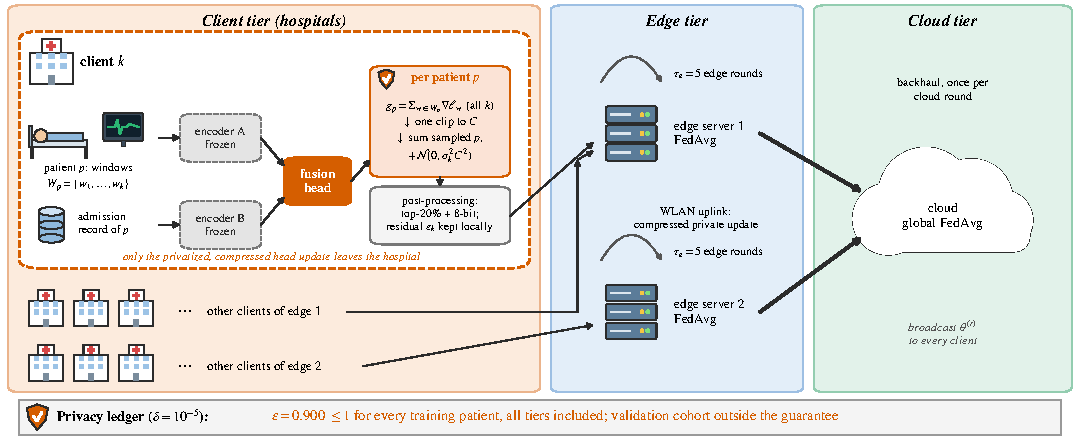
\includegraphics[width=\textwidth]{fig01_overview_core.pdf}
\caption{Architecture of PP-HFM. Clients train only the fusion head under patient-level DP; edges and the cloud average the noisy, compressed updates.}
\label{fig:overview}
\end{figure*}
A deployment has $K$ clients, such as hospitals, specialties or wearable
installations, assigned by a fixed public map $e(\cdot)$ to $E$ edge
aggregators, which report to one cloud aggregator (Fig.~\ref{fig:overview}). Client $k$ holds a dataset
$\mathcal{D}_k$ of $n_k$ records. Each record pairs two modalities of the same
individual over the same interval: modality~A is a multichannel time series
and modality~B a static or summarized feature vector. The records of client
$k$ are partitioned by individual into the patient set $\mathcal{P}_k$; patient
$p$ contributes the records $W_p$, with $k_p = |W_p|$. A patient's records
never span two clients or two evaluation splits; this holds by construction
for the eICU privacy-cost and end-to-end configurations, run on a
one-hospital-per-person partition, and for the person-level VitalDB partition
(Section~\ref{sec:setup}); the remaining eICU analyses use the source partition
and are qualified in Section~\ref{sec:method:analysis}. The model
$f_\theta$, with $\theta = (\theta_{\mathrm{enc}}, \theta_{\mathrm{head}})$,
comprises two modality encoders and a fusion head, and the learning objective
is the weighted empirical risk
\begin{equation}
\min_{\theta}\; F(\theta) = \sum_{k=1}^{K} \frac{n_k}{n}\,
\frac{1}{n_k}\!\!\sum_{(x,y)\in\mathcal{D}_k}\!\! \ell\big(f_\theta(x), y\big),
\label{eq:objective}
\end{equation}
with $n = \sum_k n_k$ and $\ell$ the unweighted cross-entropy; class weights
computed from training labels would be a further unprotected release.
Training runs for $R$ cloud rounds of $\tau_e$ edge rounds each.

Table~\ref{tab:notation} summarizes the notation.

\begin{table}[!t]
\centering
\caption{Notation}
\label{tab:notation}
\small
\begin{tabular}{ll}
\toprule
Symbol & Meaning \\
\midrule
$K$, $E$               & number of clients, of edge aggregators \\
$\mathcal{P}_k$, $W_p$ & patients of client $k$; records of patient $p$ \\
$k_p = |W_p|$          & records contributed by patient $p$ \\
$R$, $\tau_e$          & cloud rounds; edge rounds per cloud round \\
$B$, $q_k$             & expected patients per step; sampling rate \\
$C$, $\sigma_k$        & clipping norm; noise multiplier of client $k$ \\
$T_k$                  & optimization steps of client $k$ \\
$(\varepsilon,\delta)$ & privacy budget \\
\bottomrule
\end{tabular}
\end{table}

\subsection{Threat Model and Privacy Goal}
The adversary observes everything that leaves a client: every encoded update,
and every edge and cloud model. It may also
know all records except those of a target individual. Edge and cloud
aggregators are honest-but-curious and are treated as part of the adversary.
The goal is $(\varepsilon,\delta)$-differential privacy \cite{ref8} under the
\emph{patient-level} neighbouring relation: two datasets are neighbours if one
is obtained from the other by adding or removing \emph{all} records of a
single patient. A record-level guarantee, which removes one record, does not
meet this goal when $k_p > 1$. Public quantities are the architecture, the
pretrained encoder parameters, all hyperparameters, the edge map, the declared client
sizes $|\mathcal{P}_k|$ and $n_k$, and the input standardization constants,
which are fixed before training and are public only when fitted on the
disjoint pool (Table~\ref{tab:ledger}). The validation cohort, used to select the
reported checkpoint, is outside the guarantee, as is conventional
\cite{ref6}; Section~\ref{sec:method:analysis} lists every release.

\subsection{Research Objectives}
To make the three requirements testable, seven quantitative targets were fixed
before any experiment was run:
\begin{IEEEdescription}[\IEEEsetlabelwidth{O2b:}]
\item[O1:] reduce uplink traffic by at least $50\,\%$ relative to centralized
training;
\item[O1b:] reduce the latency of a training round relative to centralized
training;
\item[O2a:] keep the privacy budget at $\varepsilon \le 1$ for every protected
individual;
\item[O2b:] lose at most two points of utility relative to an identical
non-private system (cost = non-private minus private; a negative cost means
the private system scores higher);
\item[O3a:] keep the $95$th-percentile inference latency below $100$~ms;
\item[O3b:] deliver more than $99\,\%$ of updates; and
\item[O4:] save at least $20\,\%$ of energy per training round.
\end{IEEEdescription}
Section~\ref{sec:results:objectives} reports each target on every corpus.

\section{The PP-HFM Framework}
\label{sec:method}

\subsection{Overview}
\label{sec:method:overview}
Fig.~\ref{fig:overview} shows the architecture of PP-HFM. It has three
tiers: clients, which hold the patients' records; edge aggregators, each
serving a group of clients; and a cloud aggregator. Each client holds
patient-grouped multimodal records that never leave the institution. A
training round proceeds in four stages, each described in one of the
following subsections.
\begin{enumerate}
\item \emph{Local encoding.} The client passes each record through two
frozen, pretrained encoders, one per modality.
\item \emph{Patient-level private training} (Section~\ref{sec:method:privacy}).
The client trains only the fusion head, grouping each patient's gradients
before clipping and adding noise.
\item \emph{Per-client noise calibration} (Section~\ref{sec:method:calib}).
Before training, each client sets its noise level from its own population
size, so that every patient receives the same budget.
\item \emph{Hierarchical aggregation} (Section~\ref{sec:method:agg}). The
client sends a sparsified, quantized head update to its edge; each edge
averages its clients' updates for $\tau_e$ rounds and then reports to the
cloud, which averages across edges and broadcasts the global model.
\end{enumerate}
Section~\ref{sec:method:analysis} then proves the guarantee and
Section~\ref{sec:method:mia} describes how it is audited. The encoder
architecture and the averaging rule are adopted from established work; the
contribution lies in the unit at which privacy is enforced and in the
accounting of the reported budget.


\emph{Frozen multimodal backbone.} As shown in Fig.~\ref{fig:backbone}, the
temporal encoder applies three parallel
one-dimensional convolutions with different kernel widths, a strided
convolution, a further convolution with max pooling, a two-layer
bidirectional recurrent layer and attention pooling; the static encoder is a
two-layer perceptron. The two
embeddings are concatenated and mapped to class logits by the fusion head
which holds $559{,}874$ of the $1{,}864{,}227$ parameters ($30.0\,\%$). Every
normalization layer is a group or layer normalization: batch normalization
mixes statistics across a batch, which would make the per-patient gradient
ill-defined and the accounting invalid. The encoders are pretrained centrally
and frozen. Two configurations are distinguished. In the \emph{disjoint}
configuration, a set of individuals is reserved before federated training,
verified disjoint from every client's splits, and used alone for pretraining;
with standardization constants also fitted on that pool, this configuration
satisfies the guarantee end to end. In the \emph{oracle}
configuration, the encoders are pretrained on the pooled client training data;
it does not satisfy the guarantee end to end and is used only to isolate the
behavior of the private head, so its utilities are upper bounds.

\begin{figure*}[!t]
\centering
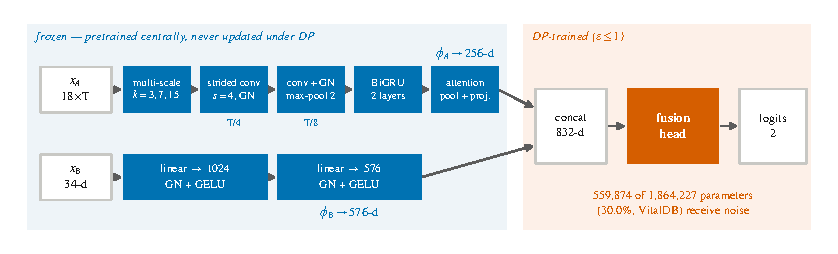
\includegraphics[width=\textwidth]{fig2_backbone.pdf}
\caption{Encoder--fusion backbone (VitalDB). Encoders are pretrained and frozen; only the fusion head ($559{,}874$ parameters) is privatized.}
\label{fig:backbone}
\end{figure*}

\subsection{Patient-Level Private Training}
\label{sec:method:privacy}
This stage ensures that each patient, and not each record, has bounded
influence on the model. The mechanism fixes the unit at the point of clipping
rather than recovering it afterwards; Fig.~\ref{fig:unit}(a) contrasts the
two. At each optimization step, client $k$
draws a Poisson sample $S \subseteq \mathcal{P}_k$, including each patient
independently with probability
\begin{equation}
q_k = \min\big(1,\ B/|\mathcal{P}_k|\big),
\label{eq:q}
\end{equation}
where $B$ is the expected number of patients per step. For each sampled
patient, the gradients of all of that patient's records are summed and the sum
is clipped,
\begin{equation}
g_p = \!\!\sum_{(x,y)\in W_p}\!\! \nabla_{\theta_{\mathrm{head}}}\,
       \ell\big(f_\theta(x), y\big), \qquad
\bar{g}_p = g_p \min\!\Big(1, \frac{C}{\lVert g_p \rVert_2}\Big).
\label{eq:clip}
\end{equation}
Because the bound is applied to the sum, patient $p$ changes the aggregate by
at most $C$ irrespective of $k_p$; clipping each record would admit $k_p C$.
Gaussian noise scaled to the same norm is added once per step, and the result
is divided by the \emph{expected} batch size,
\begin{equation}
\tilde{g} = \frac{1}{q_k |\mathcal{P}_k|}\Big( \sum_{p \in S} \bar{g}_p
+ \mathcal{N}\big(0, \sigma_k^2 C^2 I\big) \Big),
\label{eq:noise}
\end{equation}
after which $\theta_{\mathrm{head}} \leftarrow \theta_{\mathrm{head}} - \eta
\tilde{g}$; the implementation passes $\tilde{g}$ to Adam instead, which acts
only on the released gradient and is post-processing. The divisor must not be the realized $|S|$: the noise norm reveals
the divisor, $|S|$ depends on whether a given patient is present, and
normalizing by it releases information the accountant does not cover. For the
same reason a step whose sample is empty still releases the noise.
Algorithm~\ref{alg:patientdp} states the procedure. For compute, at most
$64$ records of a patient enter $g_p$; the rule is fixed and public, so the
guarantee is unaffected, and it truncates $4.1\,\%$ of eICU patients
($3.5\,\%$ of training windows) and no VitalDB patient.

\emph{Objective solved.} Without clipping, the expected step is
$\mathbb{E}[\tilde{g}] = |\mathcal{P}_k|^{-1}\sum_{p}g_p
= \bar{k}_k\,\nabla F_k(\theta)$, where $F_k$ is the record mean of
\eqref{eq:objective} on client $k$ and $\bar{k}_k = n_k/|\mathcal{P}_k|$.
A local pass takes $|\mathcal{P}_k|/B$ such steps, $\bar{k}_k$ times fewer
than a record-level pass with $B$ records per step, so to first order in
$\eta$ both displace client $k$ by $\eta\,(n_k/B)\,\nabla F_k$: before
clipping the patient-level mechanism targets \eqref{eq:objective} with
unchanged client weights, in fewer and larger steps. The argument is for the
plain gradient step; Adam rescales coordinates adaptively, so in the
implementation it holds only approximately. Clipping is what changes
the objective: each patient's summed gradient is bounded as a whole, the
surrogate of user-level DP-SGD \cite{ref11}, which down-weights patients
whose summed gradient exceeds $C$, typically those with many records. This
change belongs to the unit and is part of its measured cost
(Section~\ref{sec:results:k}).

\begin{figure}[!t]
\centering
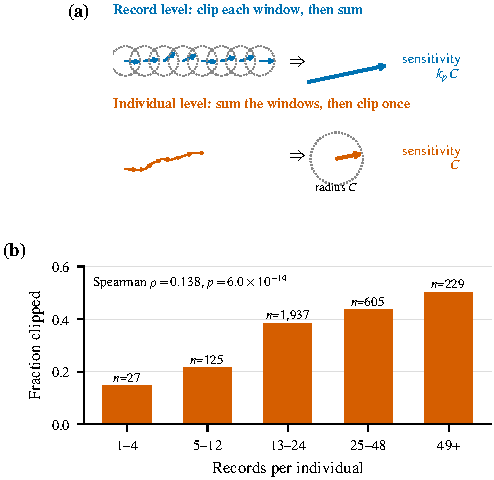
\includegraphics[width=\columnwidth]{fig02_privacy_unit.pdf}
\caption{Unit of the guarantee. (a) Per-window versus per-patient clipping. (b) Fraction of eICU individuals clipped at $C = 1$ against records contributed.}
\label{fig:unit}
\end{figure}

\begin{algorithm}[!t]
\caption{Patient-level private local update at client $k$}
\label{alg:patientdp}
\begin{algorithmic}[1]
\REQUIRE frozen $\theta_{\mathrm{enc}}$; head $\theta_{\mathrm{head}}$;
         patients $\mathcal{P}_k$ with records $\{W_p\}$; clip $C$;
         multiplier $\sigma_k$ from \eqref{eq:sigma}; rate $q_k$ from
         \eqref{eq:q}; step size $\eta$
\FOR{each local step}
  \STATE Sample $S \subseteq \mathcal{P}_k$, each $p$ independently w.p. $q_k$
  \FOR{$p \in S$}
    \STATE $g_p \leftarrow \sum_{(x,y)\in W_p}
            \nabla_{\theta_{\mathrm{head}}} \ell(f_\theta(x),y)$
            \hfill $\triangleright$ group by patient
    \STATE $\bar g_p \leftarrow g_p \cdot \min(1, C/\lVert g_p\rVert_2)$
            \hfill $\triangleright$ bound the sum
  \ENDFOR
  \STATE $\tilde g \leftarrow \big(\sum_{p\in S}\bar g_p
          + \mathcal{N}(0,\sigma_k^2C^2I)\big)/(q_k|\mathcal{P}_k|)$
          \hfill $\triangleright$ also if $S=\emptyset$
  \STATE $\theta_{\mathrm{head}} \leftarrow \theta_{\mathrm{head}} - \eta\,\tilde g$
\ENDFOR
\RETURN $\theta_{\mathrm{head}}$
\end{algorithmic}
\end{algorithm}

\subsection{Per-Client Noise Calibration}
\label{sec:method:calib}
This stage sets how much noise each client adds. Clients partitioned by
institution differ greatly in size, and therefore in
sampling rate: a small client samples a large fraction of its patients per
step. A single multiplier calibrated for the most demanding client satisfies
the budget everywhere but imposes that client's noise on all others; on eICU,
a hospital of fifteen patients sampled at $q_k = 1$ would set the noise of all
$187$ clients. When each patient is held by exactly one client (A1), the
clients' mechanisms act on disjoint individuals, and by parallel composition a
patient's guarantee is that of the client holding them; individuals held by
several clients are treated in the scope statement of Section~\ref{sec:method:privacy}. Each client therefore
uses the smallest multiplier that meets the training budget for its own
sampling rate and step count,
\begin{equation}
\begin{aligned}
\sigma_k &= \min\big\{\sigma :\ \varepsilon_k(\sigma, q_k, T_k) \le \varepsilon\big\},\\
T_k &= R\,\tau_e \max\big(1, \lfloor |\mathcal{P}_k|/B \rfloor\big),
\end{aligned}
\label{eq:sigma}
\end{equation}
where $\varepsilon_k$ is computed by the privacy loss distribution accountant
\cite{ref33}, a tight upper bound for the subsampled Gaussian mechanism, and
$T_k$ must equal the number of steps the client actually executes. Since
$\sigma_k$ depends only on the declared, public $|\mathcal{P}_k|$ and $T_k$,
using a different multiplier per client releases nothing further. Arm-versus-arm
comparisons in Section~\ref{sec:results} use the single conservative
multiplier $\sigma^{\star} = \max_k \sigma_k$ with R\'enyi accounting
\cite{ref7, ref29}, which holds every arm to the same noise.

\subsection{Hierarchical Aggregation and Update Encoding}
\label{sec:method:agg}
This stage combines the clients' private updates while keeping the uplink
small. Within a cloud round $r$, each client initializes from its edge model,
performs one private local pass, and transmits its encoded update. Edge $e$
and the cloud compute
\begin{equation}
\theta_e^{(r,s)} = \!\!\sum_{k:e(k)=e}\!\!\frac{n_k}{N_e}\,\theta_k^{(r,s)},
\qquad
\theta^{(r)} = \sum_{e=1}^{E}\frac{N_e}{n}\,\theta_e^{(r,\tau_e)},
\label{eq:agg}
\end{equation}
with $N_e = \sum_{k:e(k)=e} n_k$ (Algorithm~\ref{alg:round}). The weights
are public constants; weights
computed from the records drawn in a round would depend on which patients were
sampled and would leave the client unprotected. With $\tau_e = 1$ the edge
tier collapses into conventional single-tier federated averaging. Each update
$\Delta$ of dimension $d$ is sparsified to its $\kappa d$ largest-magnitude
coordinates and the retained values are uniformly quantized to $b$ bits,
\begin{equation}
Q(v) = v_{\min} + \operatorname{round}\!\Big(\frac{v - v_{\min}}{s}\Big)\, s,
\qquad s = \frac{v_{\max}-v_{\min}}{2^{b}-1},
\label{eq:quant}
\end{equation}
with the suppressed residual accumulated locally and added to the next
update. Both operations act on the already-perturbed head and are
post-processing.

\begin{algorithm}[!t]
\caption{PP-HFM cloud round $r$}
\label{alg:round}
\begin{algorithmic}[1]
\REQUIRE global model $\theta^{(r-1)}$; edge map $e(\cdot)$; edge rounds $\tau_e$
\STATE $\theta_e^{(r,0)} \leftarrow \theta^{(r-1)}$ for every edge $e$
\FOR{$s = 1$ \TO $\tau_e$}
  \FOR{each client $k$ \textbf{in parallel}}
    \STATE $\theta_k^{(r,s)} \leftarrow$ Algorithm~\ref{alg:patientdp}
           from $\theta_{e(k)}^{(r,s-1)}$
    \STATE transmit $Q\big(\text{top-}\kappa(\theta_k^{(r,s)}-\theta_{e(k)}^{(r,s-1)})\big)$
  \ENDFOR
  \STATE each edge aggregates by \eqref{eq:agg} (left)
\ENDFOR
\STATE cloud aggregates by \eqref{eq:agg} (right) and broadcasts $\theta^{(r)}$
\RETURN $\theta^{(r)}$
\end{algorithmic}
\end{algorithm}

\subsection{Privacy Analysis}
\label{sec:method:analysis}
This subsection proves that, under three conditions, the procedure above
protects every training patient, states what the protection costs, and lists every quantity the
system releases. Three conditions are assumed. (A1) Each patient's records lie in the training
split of exactly one client, and the training cohort is disjoint in patients
from the validation cohort, which serves checkpoint selection. (A2) The architecture, the encoder
parameters, which are pretrained on a patient-disjoint pool, all
hyperparameters, the edge map, the standardization constants and the
declared client sizes $|\mathcal{P}_k|$ and $n_k$ are public and fixed before
training; $q_k$, $T_k$, $\sigma_k$ and the weights of \eqref{eq:agg} are
computed from them and never from the data. (A3) The forward pass of a record depends on that record
alone.

\begin{theorem}[Patient-level guarantee]
\label{thm:guarantee}
Under (A1)--(A3), let each $\sigma_k$ satisfy \eqref{eq:sigma}. The transcript
of a PP-HFM run, consisting of every encoded client update, every edge and
cloud model and the model selected on the validation cohort, is
$(\varepsilon,\delta)$-differentially private with respect to each
training patient, under adding or removing all records of one patient with
the parameters of (A2) held fixed.
\end{theorem}

\begin{IEEEproof}
Fix a training patient $p$, held by client $k$ by (A1). \emph{One step.} Given
the model entering a step, the clipped gradients $\bar g_{p'}$, $p' \neq p$,
are unaffected by $p$ by (A3), and $\lVert \bar g_p\rVert_2 \le C$ by
\eqref{eq:clip}. The noisy sum in \eqref{eq:noise} is therefore a
Poisson-subsampled Gaussian mechanism with rate $q_k$, noise $\sigma_k C$ and
$\ell_2$-sensitivity $C$, whose privacy loss is bounded in
\cite{ref29, ref33}; division by the public constant $q_k|\mathcal{P}_k|$ and
the update are post-processing. \emph{Composition.} Each step takes as input
earlier outputs, other clients' messages and public quantities, so the $T_k$
steps compose adaptively, and \eqref{eq:sigma} ensures $\varepsilon_k \le \varepsilon$ at $\delta$. \emph{Other clients.} By (A1) no
other client accesses the records of $p$; its outputs are randomized
functions of its own data and of already-released messages and contribute no
privacy loss with respect to $p$. Since $\sigma_{k'}$ depends only on public
quantities, the per-client multipliers release nothing. \emph{Hierarchy.}
Sparsification with a local residual, quantization, averaging with the public
weights of \eqref{eq:agg} and broadcast are functions of released outputs and
public quantities, and selection on the validation cohort uses data disjoint
from $p$; all are post-processing.
\end{IEEEproof}

\emph{Adjacency and public sizes.} Adding or removing a patient changes the
realized cohort, but not the mechanism: the rate, step count, multiplier,
divisor and aggregation weights are fixed by the declared sizes before
training, so both neighbouring datasets are processed by the same mechanism.
This is the setting in which the Poisson-subsampled Gaussian is analyzed
\cite{ref29, ref33}; it needs no knowledge of the realized dataset and its
guarantee holds for a dataset of any size. The declared sizes are themselves
released. In the experiments they equal the realized cohort sizes, which
institutions typically publish; where a size is sensitive, it can be replaced
by a coarse public value or released by a private count at a small additional
budget, and the theorem holds for whichever declared values are used. \emph{Standardization.} The theorem holds with the standardization
constants fixed, like the declared sizes; with the constants recomputed after
a patient is removed, every other record would be represented differently.
In the experiments the constants are fitted once on the training cohort, so
their release is outside the guarantee (Table~\ref{tab:ledger}). Its size was
measured on eICU, where the fit can be reproduced exactly: removing one
individual moves any mean by at most $0.0017$ standard deviations and, for
$99\,\%$ of individuals, any standard deviation by at most $0.02\,\%$, but
the most extreme outlier moves one channel's standard deviation by
$5.2\,\%$. Constants fitted on the disjoint pretraining pool alone differ
from those used by at most $0.026$ standard deviations in mean and
$4.4\,\%$ in scale. On eICU the headline is therefore repeated with
constants fitted on the disjoint pool and encoders pretrained in those units
(Section~\ref{sec:results:privacy}); there every input to the private head is
either public or covered by the theorem.

Table~\ref{tab:ledger} lists every release of the headline configuration;
the unit comparison and the audit use $\varepsilon = 1.0 + 0.5$ with one
worst-client multiplier (Table~\ref{tab:scope}). The protected population is
the training cohort; validation patients select the checkpoint without noise
and are outside the guarantee, as is conventional \cite{ref6}.

\begin{table}[!t]
\centering
\caption{Privacy ledger of the headline configuration: every release and the
population it touches. Table~\ref{tab:scope} gives the other configurations.}
\label{tab:ledger}
\setlength{\tabcolsep}{2.4pt}
\footnotesize
\begin{tabular}{lll}
\toprule
Release & Population & Protection \\
\midrule
Client updates, edge/cloud models & training & $(0.9, 10^{-5})$-DP per client \\
Selected checkpoint               & validation & none \\
Conformal threshold (evaluated)   & validation & $\varepsilon_{\mathrm{conf}} = 0.1$ \\
Standardization (headline runs) & training & none \\
Standardization (eICU rerun) & public pool & public \\
Declared sizes, $q_k$, $T_k$, $\sigma_k$ & -- & public by design \\
Encoders (disjoint pool)          & external & not required \\
Encoders (oracle)                 & training & violates (A2) \\
\bottomrule
\end{tabular}
\end{table}

% Table IV (scope) is defined here, beside Table III, so the full-width float
% reaches the top of the page that explains it (it lands one page after definition).
\begin{table*}[!t]
\centering
\caption{Scope of the guarantee in each evaluated configuration}
\label{tab:scope}
\footnotesize
\setlength{\tabcolsep}{4pt}
\begin{tabular}{>{\raggedright\arraybackslash}p{4.8cm}>{\raggedright\arraybackslash}p{2.3cm}>{\raggedright\arraybackslash}p{3.6cm}>{\raggedright\arraybackslash}p{3.3cm}>{\raggedright\arraybackslash}p{2.7cm}}
\toprule
Configuration & Unit & Encoders / standardization & Accounting & Guarantee covers \\
\midrule
eICU, headline (one hospital per person) & patient & disjoint / training cohort & $\sigma_k$, PLD; $0.9 + 0.1$ & training transcript \\
eICU, pool-fitted constants (one hospital per person) & patient & disjoint / public pool & $\sigma_k$, PLD; $0.9 + 0.1$ & end to end \\
VitalDB, person-level headline & person & oracle / training cohort & $\sigma_k$, PLD; $0.9 + 0.1$ & transcript; (A2) violated \\
VitalDB, disjoint encoders (case-level) & surgical case & disjoint / training cohort & $\sigma_k$, PLD; $0.9 + 0.1$ & transcript, per case \\
VitalDB, cost of the unit and audit (person-level) & person vs record & oracle / training cohort & $\sigma_{\max}$, RDP; $1.0 + 0.5$ & training transcript \\
Scaling grids, clipping rule (VitalDB case-level; eICU) & individual vs record & oracle (VitalDB), disjoint (eICU) / training & $\sigma_{\max}$, RDP; $0.8$--$1.0 + 0.2$--$0.5$ & training transcript$^{\ddagger}$ \\
eICU, prior systems (source partition) & patient & disjoint / training cohort & $\sigma_k$, PLD; $0.9 + 0.1$ & training transcript$^{\ddagger}$ \\
WEAR & record (= participant) & oracle / training cohort & record-level; $0.766 + 0.2$ & transcript, per record \\
\bottomrule
\end{tabular}
\tabnote{Unit: neighboring datasets differ by all records of one patient, person or case, or by one record; ``vs'' marks a comparison of two arms. Accounting: $\varepsilon_{\mathrm{train}} + \varepsilon_{\mathrm{conf}}$ at $\delta = 10^{-5}$; $\sigma_k$, per-client multipliers; $\sigma_{\max}$, one worst-client multiplier; PLD, privacy-loss-distribution accountant; RDP, R\'enyi accountant. The conformal release was evaluated and is not part of the deployed system. Arms compared with each other share one configuration. Other analyses (recipe, ablation, fusion, attribution) are labeled with their partition and mechanism in Section~\ref{sec:results}. $^{\ddagger}$eICU on the source partition: for the $97.1\,\%$ of training persons at one hospital; the $2.9\,\%$ at two to four hospitals compose the mechanisms of those hospitals ($\varepsilon_{\mathrm{train}} \le 1.32$--$1.92$ with $\sigma_k$ and PLD).}
\end{table*}

\begin{corollary}[Coincidence of the units]
\label{cor:k1}
If every patient contributes one record, Algorithm~\ref{alg:patientdp} is
DP-SGD with Poisson sampling over records. For equal $(B, T_k, \sigma, C)$,
the patient- and record-level mechanisms are then the same mechanism, so any
difference between them at one record per patient measures seed variation or
an implementation difference, not the privacy unit.
\end{corollary}

The theorem bounds what the guarantee reveals; the next statement predicts
what it costs. Suppose $P$ individuals each contribute exactly $k$ records.
The record-level arm minimizes $\frac{1}{Pk}\sum_p\sum_{w\in W_p}\ell_w$, and
the patient-level arm minimizes the same objective written as
$\frac{1}{P}\sum_p \bar\ell_p$ with $\bar\ell_p = \frac{1}{k}\sum_{w\in
W_p}\ell_w$.

\begin{proposition}[Cost in records per individual]
\label{prop:scaling}
Let each $\ell_w$ be convex and $L$-Lipschitz on a domain of diameter $D$ in
$\mathbb{R}^d$, and let both arms be trained by private gradient descent at
the same $(\varepsilon,\delta)$, and let $\Lambda =
LD\sqrt{d\log(1/\delta)}/\varepsilon$. (i) The excess empirical risk of the
record-level arm is at most $c_{\mathrm{rec}}\Lambda/(Pk)$ and that of the
patient-level arm at most $c_{\mathrm{ind}}\Lambda/P$, with constants
independent of $k$; both rates are tight in the worst case up to logarithmic factors. (ii) If both arms
attain their rate with a common constant $c$, the gap is $A(1 - 1/k)$ with
$A = c\Lambda/P$.
\end{proposition}

\begin{IEEEproof}
For $n$ units with convex $L$-Lipschitz losses, private gradient descent
attains excess risk $O(LD\sqrt{d\log(1/\delta)}/(n\varepsilon))$, and the rate
is tight up to logarithmic factors \cite{ref31}. The record-level arm has $n = Pk$ units. In the
patient-level arm the unit is $\bar\ell_p$, which is $L$-Lipschitz as an
average of $L$-Lipschitz losses; clipping the summed gradient at $C$ equals
clipping the gradient of $\bar\ell_p$ at $C/k$, a rescaling that leaves the
guarantee unchanged, so the mechanism is private gradient descent over $n = P$
units. This gives (i), and (ii) follows by subtraction.
\end{IEEEproof}

Part (ii) rests on an assumption that (i) does not supply: upper bounds with
different constants do not determine the attained gap. The form
$A(1-1/k)$ is therefore a \emph{scaling hypothesis} that the proposition
motivates, not a theorem, and it is tested empirically, including out of
sample. Since the head is not convex and the reported metric is not excess
risk, the hypothesis concerns the \emph{shape} of the cost, not its
magnitude: one free parameter, zero at $k = 1$, and a patient-level arm whose
utility does not depend on $k$. It also indicates what would recover
the cost: mechanisms that clip around an estimate of each individual's mean
gradient attain user-level rates that improve with $k$ \cite{ref32}, whereas
a bound fixed around zero cannot.

\emph{Scope.} On eICU and on the person-level VitalDB partition the unit is
the person. On the case-level VitalDB partition it is the surgical case:
$230$ of $5{,}974$ people ($3.9\,\%$) underwent more than one operation, and
for them the guarantee extends to the person only by group privacy over at
most $14$ cases, composed across clients for the $68$ training persons whose
cases lie on two. On eICU, where clients are hospitals, the stays of $2{,}177$ of $74{,}327$ training persons ($2.9\,\%$) lie at two to four hospitals, so in the source partition (A1) fails for them. The privacy-cost and end-to-end runs therefore use a partition in which each such person is moved, with all their records, to the hospital holding most of their stays ($49{,}939$ training records; likewise $509$ validation and $589$ test persons); no record is excluded and every split is unchanged. In that partition every training and validation person is held by one hospital, so (A1) holds and the guarantee is $\varepsilon_{\mathrm{train}} = 0.9$ for every training person, verified independently for every client of every run (privacy-loss-distribution bounds $[0.880, 0.900]$; R\'enyi accountant $0.974$), and the evaluated conformal release adds $\varepsilon_{\mathrm{conf}} = 0.1$ once per person. The remaining eICU analyses (system objectives other than O2, scaling grid, clipping rule and prior systems) use the source partition, in which the per-client budget composes across the hospitals that hold a person: with the headline accountant, at most $1.32$, $1.64$ and $1.92$ for the $2{,}097$, $75$ and $5$ persons at two, three and four hospitals (R\'enyi: $1.42$, $1.77$, $2.08$), and at most $m\varepsilon$ in general; arms compared with each other share the partition. On WEAR each client is one participant, client-, user- and
record-level units coincide at the client, and the mechanism evaluated there
is record-level. The guarantee holds end to end only with the disjoint
encoders and pool-fitted standardization constants; the oracle encoders
violate (A2), and training-fitted constants are an unprotected release. Table~\ref{tab:scope} lists, for each evaluated configuration, the unit,
the provenance of the encoders and standardization constants, the accounting
and what the guarantee covers. The implementation of the accounting is
additionally checked by a suite of 17 regression checks, seven of which cover
it: composition of the budget across calls, release and accounting of noise at
every step with the expected-batch divisor, one conformal score per calibration
patient, and per-client multipliers within the budget. These are
implementation-level checks of the accounting configuration; they do not by
themselves establish the guarantee.


\subsection{Empirical Audit}
\label{sec:method:mia}
A proof bounds what an adversary can learn; an audit measures what a concrete
attack actually achieves. The guarantee is audited by patient-level membership inference. Members are
training patients and non-members are held-out patients, scored by the same
released model. Two attacks are used: thresholding of a patient's mean loss
\cite{ref15}, and LiRA \cite{ref17} adapted to the patient unit. Sixteen
shadow models are trained on independently drawn halves of the patient
population, with all records of a patient assigned together. For each patient,
the logit-scaled confidence averaged over their records,
\begin{equation}
\varphi(p) = \frac{1}{k_p}\sum_{(x,y)\in W_p}
\Big( z_y(x) - \log\!\sum_{j \neq y} e^{z_j(x)} \Big),
\label{eq:phi}
\end{equation}
is modeled by Gaussians fitted over the shadows that include and exclude the
patient (Fig.~\ref{fig:lira}), and membership is scored by
$\Lambda(p) = \log \mathcal{N}(\varphi;\mu_{\mathrm{in}},\sigma^2_{\mathrm{in}})
- \log \mathcal{N}(\varphi;\mu_{\mathrm{out}},\sigma^2_{\mathrm{out}})$.
A negative result is accepted only if the same procedure detects clearly
elevated leakage on a positive control, non-private training of the same head
over the same encoders. Attack AUCs are compared with a difficulty floor,
the AUC obtained by ranking patients by their mean statistic over the shadows
that exclude them, without the target model, because members and non-members
may differ in intrinsic difficulty. The audited models are the five-seed
record- and patient-level models of the unit comparison
(Section~\ref{sec:results:privacy}), trained at $\varepsilon = 1$, a slightly
weaker budget than the headline, so the audit is conservative.

\begin{figure}[!t]
\centering
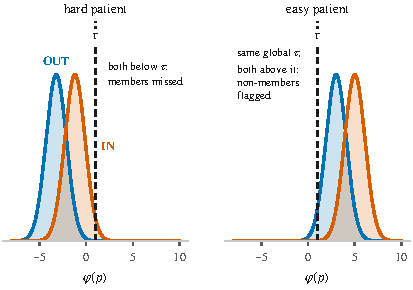
\includegraphics[width=\columnwidth]{fig4_lira.pdf}
\caption{Per-patient calibration in LiRA (illustrative): a global threshold misclassifies hard and easy patients that per-patient IN/OUT fits separate.}
\label{fig:lira}
\end{figure}

\subsection{Deployment and Instrumentation}
The trained network is exported to a portable graph and executed at full
precision on a CPU provider at the edge, so the wide-area link is not on the
inference path. Latency is decomposed into preprocessing, forward pass
and post-processing, and is reported at the
$95$th percentile over $1{,}000$ timed runs after $100$ warm-up runs.
Communication delay, delivery and traffic are measured in a packet-level
network simulation of the three tiers, with a wireless local-area
device-to-edge link and a point-to-point backhaul, on every simulated round.
Energy is modeled per tier, because a hierarchy redistributes work, and an
aggregate figure would hide a saving at one tier offset by a cost at another.

\section{Experimental Setup}
\label{sec:setup}

\subsection{Datasets}
Three public corpora are used (Table~\ref{tab:data}); Fig.~\ref{fig:workflow} outlines the study. In each, the two
modalities come from the same individual and are paired at the source rather
than by a construction rule, which a claim about fusion requires. They also
cover the two regimes that matter for the mechanism: clients holding many
individuals (VitalDB, eICU) and a client holding one (WEAR). WEAR is not
clinical: it is a wearable IoT workload that tests the system objectives
outside medicine, and its privacy results are record-level.

\begin{figure*}[!t]
\centering
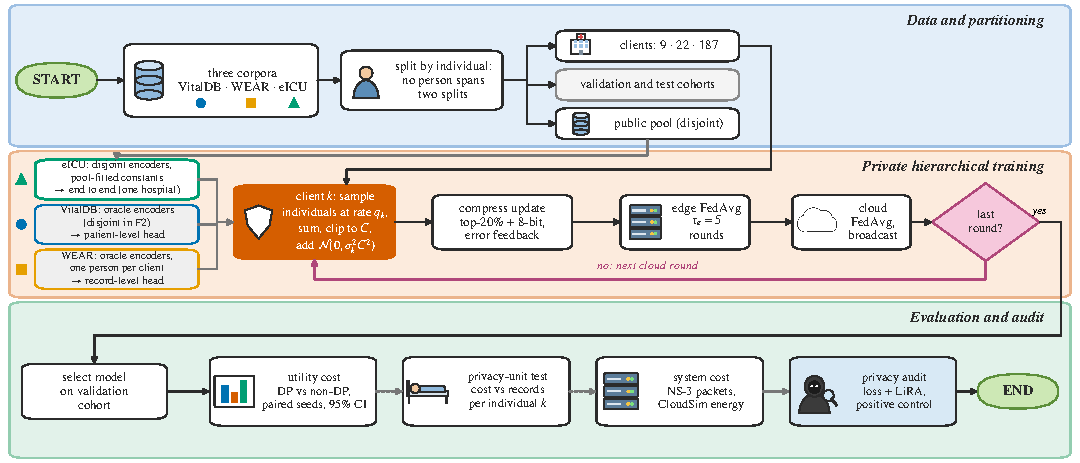
\includegraphics[width=\textwidth]{fig00_workflow.pdf}
\caption{Study workflow: individual-level partitioning, per-corpus encoder configuration (end to end on eICU only), private hierarchical training and paired evaluation with an attack audit.}
\label{fig:workflow}
\end{figure*}

\emph{VitalDB} \cite{ref20} contains non-cardiac surgical cases. Modality~A
is ten minutes of nine intraoperative trends at $0.5$~Hz with nine binary
indicators of whether each was recorded; modality~B is a $34$-dimensional
vector of preoperative clinical and laboratory variables. The target is
postoperative intensive-care admission. Clients are the nine surgical
specialties, which differ by a factor of almost eight in size and by more than
fifteen in outcome prevalence ($3.0$--$50.4\,\%$ on the person-level
partition; $3.2$--$50.7\,\%$ on the case-level partition), a
heterogeneity that arises from how care is organized rather than from an
imposed skew. \emph{WEAR} \cite{ref21}
combines body-worn inertial sensing with egocentric video features
synchronized in hardware; each of the $22$ clients is one participant.
\emph{eICU} \cite{ref27}, distributed through PhysioNet \cite{ref28} under a
credentialed agreement, is the external clinical corpus. Modality~A is the
first $24$ hours after unit admission in $60$-minute windows of six vital signs
and six observation indicators; modality~B is age, sex, admission weight and
height and the APACHE score, a clinician-computed summary rather than an
independent sensor stream; the target is in-unit mortality. Prediction is
made at hour $24$: individuals who die within the first $24$ hours are
excluded, and the APACHE score, computed from the worst values of the first
day, is therefore available at prediction time. Clients are the
hospitals themselves: of $206$, those with fewer than $200$ windows or no
positive outcome are pooled, giving $187$ clients with a median of $444$
individuals.

\begin{table}[!t]
\centering
\caption{The three corpora}
\label{tab:data}
\setlength{\tabcolsep}{2.6pt}
\small
\begin{tabular}{lccc}
\toprule
& VitalDB & WEAR & eICU \\
\midrule
Clients     & $9$ specialties & $22$ participants & $187$ hospitals \\
Ind.        & $5{,}974$ & $22$ & $132{,}736$ \\
Windows (k) & $33.5/6.8/6.9$ & $26.4/5.4/6.0$ & $2122/564/570$ \\
$\bar{k}$   & $7.9$ & ${\approx}1{,}750$ & $28.5$ \\
Modality A  & $18$-ch.\ trends & $12$-ch.\ inertial & $12$-ch.\ vitals \\
Modality B  & $34$ preop. & $2048$ video & $5$ admission \\
Task        & ICU admission & $18$ activities & mortality \\
Prevalence  & $18.84\,\%$ & -- & $4.22\,\%$ \\
\bottomrule
\end{tabular}
\tabnote{Ind.: individuals; $\bar{k}$: mean records per individual; windows are
training/validation/test, in thousands. VitalDB: person-level partition (the
case-level partition has $6{,}257$ cases, $34.0/7.3/7.4$k windows and a
prevalence of $19.65\,\%$).}
\end{table}

On eICU and WEAR, splits are made by individual. VitalDB is evaluated on two
partitions. The \emph{person-level} partition assigns each person to one
split and one client; cases that would place a person in a second split or on
a second client are removed ($200$ cases), leaving $4{,}221$ training, $868$
validation and $885$ test persons. The \emph{case-level} partition of the
earlier experiments splits by operation, so that $55$ of $940$ test persons
also have a training case and $68$ training persons span two clients; results
on it protect the case rather than the person and are marked case-level. The
privacy cost, the cost of the unit, the comparison with prior systems and the
membership-inference audit are person-level. All partitions are fixed, and no test case of either was used to
pretrain the encoders. Four controls prevent inflation that would
not be visible during training: splits by case rather than by window, which
would place near-duplicates in the test set; modality~B restricted to
preoperative variables, because intraoperative interventions are given in
response to deterioration and encode the outcome; missing values filled
within a case and paired with an explicit indicator, because, for example, an
arterial line is placed only in patients judged at risk; and normalization
statistics computed on training cases only, or on the disjoint pool for the
end-to-end eICU run. For eICU, a pool of $526{,}867$
windows from individuals disjoint from every client is reserved before
federated training to pretrain the disjoint encoders.

\subsection{Implementation}
Table~\ref{tab:params} lists the training and evaluation parameters. All arms
share one configuration, so that differences can be attributed to the factor
under test. The headline system uses per-client multipliers and the privacy
loss distribution accountant (Section~\ref{sec:method:calib}). On eICU every
pretrained encoder is disjoint. On VitalDB and WEAR, results use the oracle
encoders unless stated, so absolute utilities there are upper bounds, whereas
differences between arms, which share the encoders, are unaffected. The
trained model is exported to ONNX and timed with ONNX Runtime on the CPU
provider of a workstation (Intel Core i7-14700), not on edge hardware; the network is simulated in ns-3 and energy is modeled in
CloudSim~Plus.

\begin{table}[!t]
\centering
\caption{Training and evaluation parameters}
\label{tab:params}
\footnotesize
\setlength{\tabcolsep}{4pt}
\begin{tabular}{@{}p{0.40\columnwidth}p{0.56\columnwidth}@{}}
\toprule
Parameter & Value \\
\midrule
Cloud rounds $R$; edge rounds $\tau_e$ & $10$; $5$ \\
Edge aggregators $E$ & $2$ (eICU scaling test: $2$--$16$) \\
Local passes per edge round & $1$ \\
Optimizer & Adam \\
Learning rate; weight decay & $10^{-3}$; $10^{-4}$ \\
Expected individuals per step $B$ & $64$ \\
Clipping norm $C$ & $1$ \\
Training budget & $\varepsilon = 0.9$, $\delta = 10^{-5}$ \\
Accountant & privacy loss distribution, per-client $\sigma_k$ \\
Records per patient (cap) & $64$ \\
Update encoding & top-$20\,\%$, $8$-bit, error feedback \\
Seeds & $5$ (paired); $3$ for grids \\
LiRA shadow models & $16$ \\
Latency timing & P95, $1{,}000$ runs, $100$ warm-up \\
Software & PyTorch~2.5, Opacus~1.5, ONNX Runtime, ns-3~3.46, CloudSim~Plus~8.5 \\
Hardware & one NVIDIA RTX~A2000 GPU \\
\bottomrule
\end{tabular}
\end{table}

\subsection{Metrics and Statistics}
The primary utility measure is the area under the ROC curve (AUROC); average
precision (AUPRC) is reported because the clinical tasks are imbalanced.
Accuracy at the default threshold is uninformative under this imbalance: a
constant negative prediction attains the base rate. Balanced accuracy is
therefore reported at a threshold chosen on the validation cohort by Youden's
index. Case-level metrics average the predictions of a case's windows.
Comparisons between arms are paired by seed, and intervals are
\begin{equation}
\bar d \pm t_{S-1,\,0.975}\; s_d / \sqrt{S}
\label{eq:ci}
\end{equation}
over $S$ seeds with per-seed differences $d_s$. An effect is called
\emph{resolved} when this interval excludes zero; an unresolved estimate is
reported as such and is not read as evidence of absence. Grids run at three
seeds estimate how a cost changes across a factor, not each cell
individually. Seed counts were fixed before
each comparison and were not increased after inspecting results. The
reported checkpoint is the one with the best validation AUROC, and each is
evaluated once on the test split.

\subsection{Experimental Protocol}
\emph{System objectives} compare PP-HFM with centralized training and with the
hierarchy alone. \emph{Privacy cost} (O2b) compares the private system with
an identical non-private system over five paired seeds; the primary measure
(AUROC) and the secondary measures (AUPRC, balanced accuracy) were declared
before the runs. \emph{Recipe decomposition} uses three arms at
$\varepsilon \in \{0.5, 1, 2, 4, 8, \infty\}$: B4, full-model private training
from random initialization (prior art); B7, full-model private training from
the pretrained initialization; and B6, head-only private training from the
pretrained initialization (PP-HFM). B4$\rightarrow$B7 changes only the
initialization and B7$\rightarrow$B6 only the privatized subset.
\emph{Records per individual}: the number of training records retained per
individual, $k$, is varied with the number of units per step held equal in
both arms, which removes the sampling-rate effect and leaves only the
clipping geometry; validation and test sets are unchanged, and $k = 1$ is the
control of Corollary~\ref{cor:k1}. \emph{Ablations} remove one component at a
time. \emph{Fusion} is measured outside the federated system, each arm
retrained on its own inputs, because zeroing a stream of a jointly trained
model measures robustness rather than information.

\section{Results}
\label{sec:results}

\subsection{System Objectives}
\label{sec:results:objectives}
Table~\ref{tab:objectives} reports every objective of
Section~\ref{sec:model} on the three deployments, and Fig.~\ref{fig:system}
shows the system costs behind O1, O1b and O4. All targets are met on VitalDB.
On WEAR all are met except the utility bound, which is inconclusive. On eICU
five of seven are met; the utility bound is inconclusive under the
prespecified interval criterion, with a point estimate above it, and is
missed end to end; update delivery falls short at two edges.

\begin{table}[!t]
\centering
\caption{Objectives, measured or simulated, against the targets fixed in advance}
\label{tab:objectives}
\small
\setlength{\tabcolsep}{3pt}
\begin{tabular}{llrrrl}
\toprule
& Quantity & VitalDB & WEAR & eICU & Target \\
\midrule
O1  & Uplink reduction     & $90.8\%$   & $96.1\%$   & $92.3\%$   & $\ge 50\%$ \\
O1b & Round latency cut    & $16.9\%$   & $21.7\%$   & $33.4\%$   & $> 0\%$ \\
O2a & Budget $\varepsilon$        & $0.900$    & $0.766^{\S}$ & $0.900$  & $\le 1$ \\
O2b & Utility loss [pts]   & $-1.18$    & $1.97$~pp$^{\dagger\S}$ & $3.10^{\dagger}$ & $\le 2$ \\
O3a & P95 latency [ms]     & $2.30$     & $0.75$     & $0.24$     & $< 100$ \\
O3b & Update delivery      & $100.00\%$ & $99.94\%$  & $97.83\%^{\ast}$ & $> 99\%$ \\
O4  & Energy saving        & $72.3\%$   & $76.8\%$   & $79.6\%$   & $\ge 20\%$ \\
\bottomrule
\end{tabular}
\tabnote{Measured: inference latency on a workstation CPU (ONNX Runtime) and the
uplink payload of the deployed update encoding. Simulated: delivery and round latency (packet-level ns-3, every
round) and energy (CloudSim Plus model). O2b: paired loss against an identical non-private system, five seeds,
in AUROC points. $^{\S}$Record-level; O2b is the accuracy loss over fifteen
seeds. $^{\dagger}$Interval spans the threshold (eICU: $[1.55, 4.65]$, point
estimate above it; end to end $3.88$ $[2.60, 5.17]$, not met). $^{\ast}$Not
met. VitalDB: O2a and O2b person-level, other rows
case-level. eICU: O2a and O2b with each person at one hospital, other rows on
the source partition (Section~\ref{sec:method:privacy}). O2a: training budget; the evaluated, non-deployed conformal
release adds $\varepsilon_{\mathrm{conf}} = 0.1$ on VitalDB and eICU (total
$1.0$) and $0.2$ on WEAR (total $0.966$).}
\end{table}

\begin{figure*}[!t]
\centering
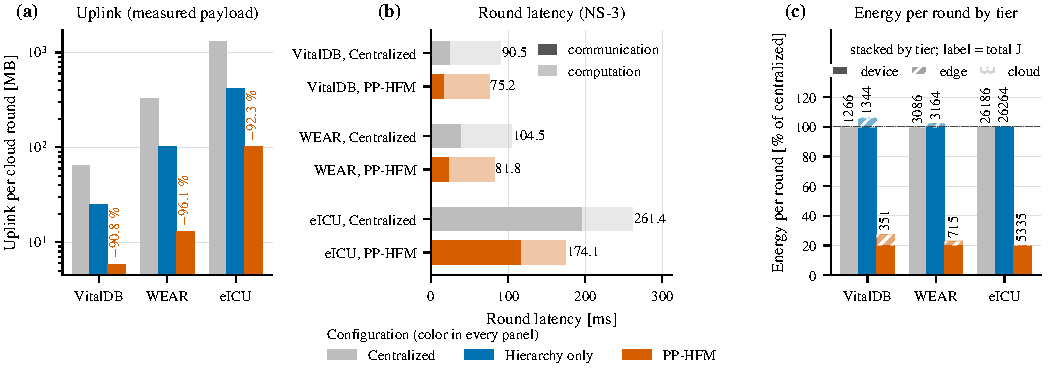
\includegraphics[width=\textwidth]{fig09_system_cost.pdf}
\caption{System cost: (a) uplink per cloud round, (b) round latency, (c) energy per round by tier, relative to centralized training.}
\label{fig:system}
\end{figure*}

\emph{Communication and latency.} Two-tier aggregation of the compressed head
update reduces uplink traffic by $90.8$, $96.1$ and $92.3\,\%$. The
measurement includes the index array that sparsification transmits with the
values, which analytical estimates omit. Round latency falls from $90.5$ to
$75.2$~ms on VitalDB, from $104.5$ to $81.8$~ms on WEAR and from $261.4$ to
$174.1$~ms on eICU, and the reduction is positive in every simulated round.
It is smaller than the traffic reduction because the hierarchy shortens link
time, not computation, and it grows with the number of stations sharing a
medium. Measuring every round at packet level matters: an earlier
configuration that composed nine rounds in ten analytically placed the
communication term of the centralized baseline at $256$~ms against $23.6$~ms
simulated, overstating the benefit fourfold.

\emph{Inference latency.} Timed on a workstation CPU (Intel Core i7-14700),
not on edge hardware, the $95$th-percentile latency is $2.30$, $0.75$ and
$0.24$~ms against a budget of $100$~ms (Table~\ref{tab:latency}). The private
mechanism adds no inference cost, because its noise acts only on training
gradients; eight-bit quantization was rejected because it raised the
$95$th percentile to $17.34$~ms.

\begin{table}[!t]
\centering
\caption{Inference latency on VitalDB ($1{,}000$ timed runs, workstation CPU)}
\label{tab:latency}
\small
\begin{tabular}{lrr}
\toprule
Stage & Mean [ms] & P95 [ms] \\
\midrule
Preprocessing              & $0.106$ & $0.110$ \\
Forward pass               & $2.130$ & $2.165$ \\
Conformal set (not deployed) & $0.019$ & $0.021$ \\
Post-processing            & $0.007$ & $0.008$ \\
\midrule
Total                      & $2.263$ & $2.299$ \\
Total, eight-bit graph     & $3.515$ & $17.337$ \\
\bottomrule
\end{tabular}
\tabnote{After $100$ warm-up runs. The eight-bit graph was evaluated and not
deployed.}
\end{table}

\emph{Reliability and energy.} Update delivery is $100.00$ and $99.94\,\%$ on
VitalDB and WEAR. On eICU, $187$ clients on two edges contend for the shared
medium, and delivery is $97.83\,\%$, against $95.11\,\%$ for centralized
training. With the edge count varied and everything else fixed, delivery
rises monotonically to $99.94\,\%$ at sixteen edges, meets the target on
average from six edges and in every round from eight (about $23$ clients per
edge, minimum $99.49\,\%$). Energy per round falls by $72.3$, $76.8$ and
$79.6\,\%$. Introducing the edge tier alone increases total energy, from
$1{,}266$ to $1{,}344$~J on VitalDB; the saving comes from the reduced device
computation and transmission of PP-HFM, which lowers the device term
fivefold.

\subsection{Privacy Budget and Utility}
\label{sec:results:privacy}
On both clinical corpora, the contribution to the training transcript of
every training patient is protected at
$\varepsilon = 0.900$, $\delta = 10^{-5}$, across all tiers; on eICU these runs
use the partition in which each person is held by one hospital
(Section~\ref{sec:method:privacy}). This is not an end-to-end guarantee for
the headline runs: their standardization constants are fitted on the
training cohort, and on VitalDB and WEAR the oracle encoders also violate
(A2) (Table~\ref{tab:ledger}). The VitalDB and WEAR results are therefore
comparisons of the private head, not end-to-end private deployments; the
only configuration that satisfies the guarantee end to end is the eICU rerun with disjoint encoders and pool-fitted constants, reported separately below. The per-client
multipliers range from $6.34$ to $15.56$ on VitalDB and from $4.85$ to
$29.34$ on eICU (median $13.76$); a single worst-case multiplier would have
imposed $29.34$ on every hospital.

\emph{A private calibration threshold.} A per-client conformal threshold
released by the exponential mechanism over ranks \cite{ref30, ref24}
($\varepsilon_{\mathrm{conf}} = 0.1$) was evaluated and is not part of the
system: with about a hundred calibration patients per client the private
threshold returns the majority-class set on every VitalDB seed and on four of
five eICU seeds, so coverage equals the base rate ($80.1\,\%$ on VitalDB,
case-level partition; $95.8\,\%$ on eICU) and misses the $90\,\%$ target.
The non-private threshold does not collapse (positive-class coverage
$36$--$43\,\%$), but its coverage, $80.4$--$81.8\,\%$, also misses the
target.

At the default threshold the private model predicts the majority class on
every VitalDB seed and on four of five eICU seeds (accuracy $0.8113$ and
$0.958$, the base rates), so accuracy measures the threshold rather than the model, and the
declared measures are used. On VitalDB the private model attains an AUROC of
$0.8318$ against $0.8200$ for the non-private reference, a change of $-1.18$
points $[-1.63, -0.73]$ ($p = 0.002$); AUPRC changes by $-3.47$
$[-6.33, -0.61]$ and balanced accuracy by $-0.31$ $[-1.23, +0.62]$, negative
values favoring the private model. O2b is met. The gain is consistent with
regularization of the compact head by clipping and noise, which the
case-level ablation suggests (Section~\ref{sec:results:ablation}) but this
experiment does not isolate; on the
case-level partition the change was $-0.90$ $[-1.82, +0.02]$. On eICU a cost is resolved: AUROC falls from
$0.8239$ to $0.7929$, by $3.10$ points $[1.55, 4.65]$; the interval spans the
two-point target, so O2b is inconclusive under the prespecified interval
criterion at five seeds, although the point estimate exceeds the target. AUPRC falls by $1.84$ $[1.60, 2.08]$, spanning the
threshold, and balanced accuracy by $0.33$ $[-0.22, +0.88]$, which meets it.
The cost is set by the smallest hospitals, which sample every patient at every
step and carry the largest multipliers. With standardization constants
fitted on the disjoint pool and encoders pretrained in those units, so that
the guarantee holds end to end, the eICU cost is $3.88$ points
$[2.60, 5.17]$, $2.31$ $[1.42, 3.21]$ in AUPRC and $2.80$ $[2.52, 3.08]$ in
balanced accuracy: O2b is missed in AUROC and in balanced accuracy, whose
intervals lie above the target, while the AUPRC interval spans it with a point
estimate above it. Assigning each person to one hospital left the cost of
privacy unchanged within resolution: against the same arms on the source
partition, paired by seed, the AUROC cost differs by $+0.01$ $[-0.72, +0.75]$
points with training-fitted and by $-0.03$ $[-0.66, +0.60]$ with pool-fitted
constants; on the source partition the end-to-end balanced-accuracy interval,
$[1.57, 3.82]$, had spanned the target. On WEAR, whose guarantee is
record-level, the accuracy loss is $1.97$ pp $[1.76, 2.17]$, spanning the
threshold.

\emph{Cost of the unit.} Moving the guarantee from the record to the patient
at a matched budget ($\varepsilon = 1$, five seeds, VitalDB) changes AUROC by
$-0.0170$ $[-0.0269, -0.0071]$ ($0.8423 \rightarrow 0.8254$) and AUPRC by
$-0.0582$ $[-0.0701, -0.0462]$ (case-level: $-0.0147$ and $-0.0783$). Two effects
contribute: sampling patients rather than records reduces the sampled units
from $33{,}491$ to $4{,}221$, and clipping a patient's summed gradient constrains
individuals with many records most. Section~\ref{sec:results:k} isolates the
second.

\emph{Cost of disjoint encoders.} With the disjoint instead of the oracle
encoders, the VitalDB model (case-level partition) loses $1.57 \pm 0.46$ AUROC points
($0.8395 \rightarrow 0.8237$, five paired seeds, $p < 0.001$) and
$1.22 \pm 2.62$ AUPRC points, which is not resolved. Against a non-private
reference with the same disjoint encoders, the cost of privacy is
$+0.14$ $[-0.33, +0.62]$ AUROC points, which meets O2b, and $+2.21$
$[-0.03, +4.46]$ AUPRC points.
This configuration satisfies (A2), but its standardization constants are still
fitted on the training individuals; on eICU, where the disjoint pool is not
carved from a small cohort, every result already uses disjoint encoders.

\subsection{Initialization, Not the Privatized Subset}
\label{sec:results:recipe}
PP-HFM differs from conventional private training in two respects: it starts
from pretrained encoders and privatizes only the head.
Table~\ref{tab:recipe} and Fig.~\ref{fig:recipe} separate the two. On VitalDB
(case-level partition), under the patient-level mechanism, changing only the initialization is worth
$0.0129$ AUROC without noise and $0.1991$ at $\varepsilon = 0.5$, increasing
monotonically as the budget tightens; on WEAR it ranges from $0.0021$ to
$0.3580$. Under privacy, restricting the privatized subset changes AUROC by
between $-0.0059$ and $-0.0025$ on VitalDB and by at most $0.0013$ on WEAR,
with intervals covering zero at every finite budget. Only without noise does
the head-only arm score higher on VitalDB, by $0.0139 \pm 0.0124$; no privacy
mechanism is involved there.

\begin{table}[!t]
\centering
\caption{Recipe decomposition in AUROC (three seeds; VitalDB case-level)}
\label{tab:recipe}
\setlength{\tabcolsep}{3.5pt}
\small
\begin{tabular}{lcccc}
\toprule
& \multicolumn{2}{c}{VitalDB} & \multicolumn{2}{c}{WEAR} \\
\cmidrule(lr){2-3}\cmidrule(lr){4-5}
$\varepsilon$ & B4$\rightarrow$B7 & B7$\rightarrow$B6 & B4$\rightarrow$B7 & B7$\rightarrow$B6 \\
\midrule
$\infty$ & $+0.0129$ & $+0.0139 \pm 0.0124$ & $+0.0021$ & $-0.0002 \pm 0.0003$ \\
$8$      & $+0.1407$ & $-0.0025 \pm 0.0059$ & $+0.0883$ & $+0.0001 \pm 0.0002$ \\
$4$      & $+0.1569$ & $-0.0029 \pm 0.0063$ & $+0.1257$ & $+0.0001 \pm 0.0002$ \\
$2$      & $+0.1727$ & $-0.0035 \pm 0.0040$ & $+0.1918$ & $+0.0002 \pm 0.0001$ \\
$1$      & $+0.1841$ & $-0.0059 \pm 0.0063$ & $+0.2827$ & $+0.0003 \pm 0.0008$ \\
$0.5$    & $+0.1991$ & $-0.0042 \pm 0.0043$ & $+0.3580$ & $+0.0013 \pm 0.0088$ \\
\bottomrule
\end{tabular}
\tabnote{B4$\rightarrow$B7 changes only the initialization; B7$\rightarrow$B6
only the privatized subset (whole network $\rightarrow$ head). Mean $\pm$
Student-$t$ half-width. VitalDB uses the patient-level mechanism on the
case-level partition; WEAR is record-level.}
\end{table}

\begin{figure*}[!t]
\centering
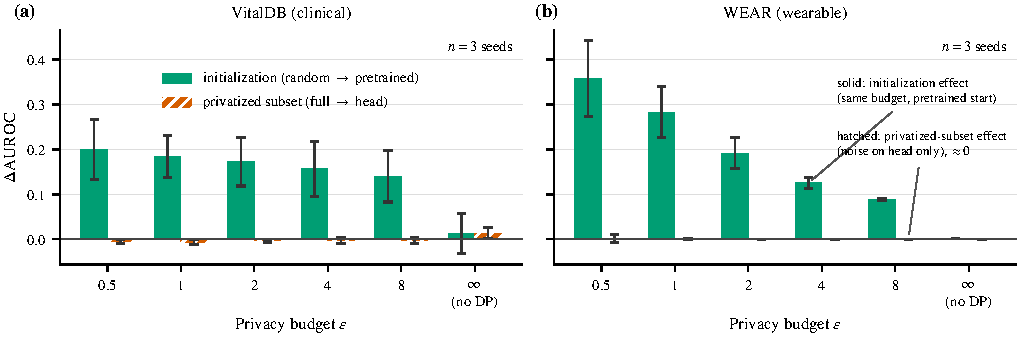
\includegraphics[width=\textwidth]{fig05_init_vs_subset.pdf}
\caption{Recipe decomposition across $\varepsilon$ (AUROC, $n = 3$, $95\,\%$ CI; VitalDB case-level): solid, initialization effect; hatched, privatized-subset effect.}
\label{fig:recipe}
\end{figure*}

The result contradicts a dimensionality explanation. If a smaller privatized
vector absorbed less noise, B7, which privatizes all $1{,}864{,}227$
parameters, should trail B6, which privatizes $559{,}874$, most at the
tightest budget. At $\varepsilon = 0.5$ the two differ by $0.0042$, within
the interval and with B7 the higher, consistent with the noise scale being set
by the budget, the step count and the sampling rate rather than by the number
of parameters. Across the budget range, the randomly initialized arm loses
$0.1906$ on VitalDB and $0.3716$ on WEAR, where it falls to $0.6247$, close to
chance; the pretrained full-model arm loses $0.0043$ and the head-only arm
$0.0225$ on VitalDB, and both less than $0.016$ on WEAR. Restricting the
subset is therefore justified by communication, since only the head is
transmitted, not by accuracy.

\subsection{Records per Individual}
\label{sec:results:k}
Table~\ref{tab:kscaling} and Fig.~\ref{fig:klaw} report the gap between the
record- and patient-level arms as the number of training records per
individual $k$ varies, with the units per step equal in both arms (VitalDB
case-level).

\begin{table}[!t]
\centering
\caption{AUPRC gap between the record and patient arms (three seeds; VitalDB case-level)}
\label{tab:kscaling}
\setlength{\tabcolsep}{3pt}
\small
\begin{tabular}{rcccc}
\toprule
& \multicolumn{2}{c}{VitalDB ($\varepsilon_{\mathrm{tr}} = 1$)} &
\multicolumn{2}{c}{eICU ($\varepsilon_{\mathrm{tr}} = 0.8$)} \\
\cmidrule(lr){2-3}\cmidrule(lr){4-5}
$k$ & Gap & $p$ & Gap & Forecast \\
\midrule
$1$  & $-0.0071 \pm 0.0599$ & $0.661$ & $-0.0011 \pm 0.0369$ & $0.0000$ \\
$2$  & $+0.0486 \pm 0.0129$ & $0.004$ & $+0.0048 \pm 0.0057$ & $0.0515$ \\
$4$  & $+0.0796 \pm 0.0163$ & $0.002$ & $+0.0081 \pm 0.0554$ & $0.0816$ \\
$8$  & $+0.0872 \pm 0.0248$ & $0.004$ & $+0.0099 \pm 0.0437$ & $0.0876$ \\
$16$ & --                   & --      & $+0.0103 \pm 0.0332$ & $0.0878$ \\
\bottomrule
\end{tabular}
\tabnote{Record arm minus patient arm, paired by seed; mean $\pm$ Student-$t$
half-width. The forecast for eICU was registered before the corpus was built.}
\end{table}

\begin{figure*}[!t]
\centering
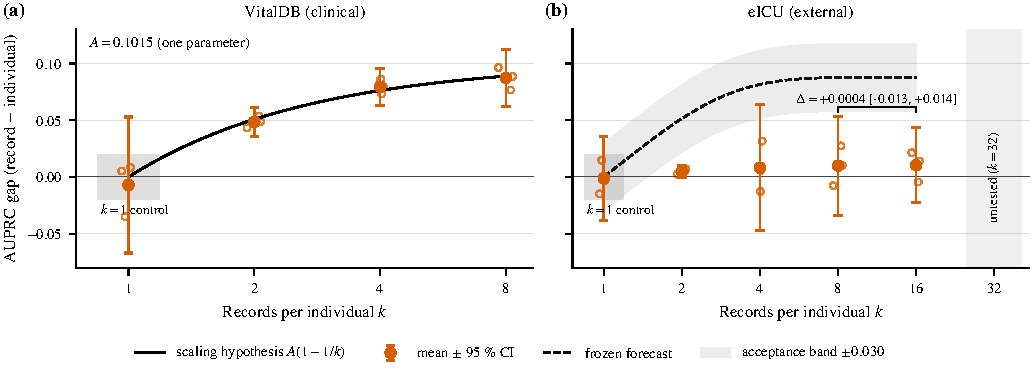
\includegraphics[width=\textwidth]{fig03_klaw.pdf}
\caption{Patient-level cost (AUPRC gap) against records per individual $k$, $n = 3$: (a) VitalDB (case-level) with the fitted curve $A(1-1/k)$; (b) eICU against the frozen forecast.}
\label{fig:klaw}
\end{figure*}

\emph{VitalDB.} At $k = 1$ the arms are indistinguishable ($-0.0071$, interval
covering zero), as Corollary~\ref{cor:k1} requires, so the divergence at
larger $k$ is attributable to the unit. From $k = 2$ the gap is resolved and
grows to $0.0872$ at $k = 8$. The patient-level arm is flat (means
$0.5083$--$0.5128$), whereas the record-level arm rises from $0.5015$ to
$0.5955$ (Fig.~\ref{fig:arms}): the widening gap is additional records that
the record-level arm exploits and the patient-level arm cannot, because the bound on the summed
contribution is tightest for the individuals who contribute them. AUROC moves
in the same direction ($+0.0026$ to $+0.0159$) but is unresolved at three
seeds.

\begin{figure}[!t]
\centering
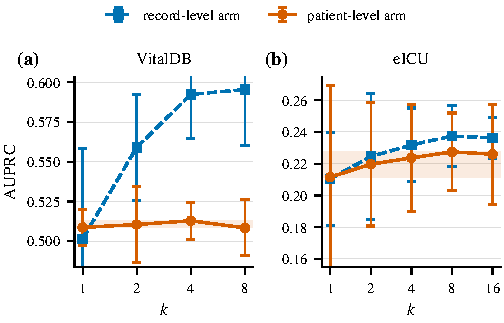
\includegraphics[width=\columnwidth]{fig04_arms.pdf}
\caption{AUPRC of each arm against $k$ ($n = 3$, $95\,\%$ CI): (a) VitalDB (case-level), where the patient-level arm is flat and the record-level arm improves; (b) eICU, where the arms overlap at every $k$.}
\label{fig:arms}
\end{figure}

\emph{Test of the scaling hypothesis.} The one-parameter curve
$A(1 - 1/k)$, fitted to the twelve paired gaps, gives $A = 0.1015$ at a
root-mean-square error of $0.0119$, against $0.0117$ for a two-parameter
saturating curve $A(1 - e^{-b(k-1)})$: the extra parameter buys nothing. Fitted
on $k \le 4$ only, it predicts $0.0904$ at $k = 8$ against $0.0872$ observed.
The patient-level arm changes by less than $0.001$ per doubling of $k$, as the
proposition requires.

\emph{External test on eICU.} Before the eICU corpus was built, a forecast was
registered from the VitalDB grid ($A = 0.0878$, $b = 0.883$) with an
acceptance band of $\pm 0.030$. On eICU the $k = 1$ control holds
($-0.0011$), and the ordering and the saturation reproduce: the gap
rises through $k = 8$ and changes by $+0.0004$
$[-0.0134, +0.0141]$ from $k = 8$ to $k = 16$, meeting the registered bound
on further growth. The magnitude does not: at $k = 8$ the gap is
$0.0099$, about one ninth of the forecast, and no eICU gap is resolved
at three seeds. Attainable precision differs by a factor of two between the
tasks (AUPRC near $0.22$ at a prevalence of $4.2\,\%$, against $0.5$), and a
cost that is a fixed fraction of attainable precision would preserve the
shape at a lower ceiling; distinguishing this from a corpus-specific ceiling
requires a third corpus. The registered design extended to $k = 32$, but only
$20.2\,\%$ of eICU individuals reach $32$ records, all of them readmitted, so
the maximum was reduced to $16$ by a dated amendment before any result beyond
$k = 8$ was computed.

\emph{Budget confound.} The forecast was fitted at
$\varepsilon = 1$ and tested at $0.8$ with a batch of $64$.
Re-running VitalDB at the eICU operating point (Table~\ref{tab:matched})
does not shrink its gaps ($+0.0914$ against $+0.0872$ at $k = 8$; the
one-parameter curve fitted on $k \le 4$ predicts $0.0988$), so the budget does
not explain the shortfall. That grid,
however, fails its own $k = 1$ control ($+0.0398$, all seeds of one sign),
which combines the smallest training pool with the largest batch; subtracting
each grid's $k = 1$ offset attributes about half ($51\,\%$) of the
difference at $k = 8$ to the operating point, and under neither reading does
the corpus term change sign.

\begin{table}[!t]
\centering
\caption{AUPRC gap across the three scaling grids (three seeds; VitalDB case-level)}
\label{tab:matched}
\setlength{\tabcolsep}{3.5pt}
\small
\begin{tabular}{ccccc}
\toprule
 & & \multicolumn{2}{c}{VitalDB} & eICU \\
\cmidrule(lr){3-4}\cmidrule(lr){5-5}
$k$ & Forecast & $\varepsilon_{\mathrm{tr}}\!=\!1.0$ & $\varepsilon_{\mathrm{tr}}\!=\!0.8$ & $\varepsilon_{\mathrm{tr}}\!=\!0.8$ \\
\midrule
$1$ & $0.0000$ & $-0.0071$ & $+0.0398$ & $-0.0011$ \\
$2$ & $0.0515$ & $+0.0486$ & $+0.0364$ & $+0.0048$ \\
$4$ & $0.0816$ & $+0.0796$ & $+0.0981$ & $+0.0081$ \\
$8$ & $0.0876$ & $+0.0872$ & $+0.0914$ & $+0.0099$ \\
\bottomrule
\end{tabular}
\tabnote{The two VitalDB grids differ only in the operating point. The forecast
was fitted on VitalDB at $\varepsilon_{\mathrm{tr}} = 1$ and never refitted.}
\end{table}

\emph{Clipping rule.} The flatness of the patient-level arm could stem from
the clipping rule rather than the unit. Normalizing each patient's summed
gradient by its record count, or its square root, before clipping leaves the
sensitivity and the budget unchanged and tests this. On the natural eICU
partition, where records per individual range from $2$ to $192$, the count
normalization lowers the final-round clipped fraction from $0.14$ to $0.08$
but changes AUPRC by $-0.0012$ $[-0.0093, +0.0069]$ (three seeds); the
one-sided $95\,\%$ upper bound, $+0.0043$, excludes the pre-registered
recovery of $+0.010$, and square-root normalization changes AUPRC by
$-0.0031$. On VitalDB at $k = 8$ and the same budget, count normalization
lowers the final-round clipped fraction from $0.50$ to $0.34$ and changes
AUPRC by $+0.0038$ $[-0.0072, +0.0148]$; the one-sided upper bound, $+0.0113$,
does not exclude $+0.010$, so this test is inconclusive by its own criterion,
and square-root normalization changes AUPRC by less than $10^{-4}$. The
clipping rule therefore does not explain the cost on eICU, and on VitalDB it
explains at most one eighth of the $0.0914$ cost at that operating point.

\subsection{Multimodal Fusion}
\label{sec:results:fusion}
On VitalDB (case-level partition) the fused model attains $0.8653 \pm 0.0072$ AUROC against
$0.8283 \pm 0.0087$ for the better single modality, a gain of $0.0370$ at
$5.9$ seed standard deviations, and $0.0671$ in AUPRC (five seeds). On WEAR
the better single modality already reaches $0.9976$, leaving no headroom. On
eICU fusion yields nothing in the natural configuration ($+0.0037$, and
$+0.0020$ on the partitions of the test below), where the admission stream
($0.8221$) dominates the vital-sign stream ($0.7068$). A
pre-registered test weakened the stronger stream to parity by mixing its
dominant feature with variance-preserving noise, calibrated on that stream
alone and never on the fused model (Table~\ref{tab:fusion},
Fig.~\ref{fig:fusion}). At parity the fused model exceeds the better single
modality by $0.0291 \pm 0.0211$, positive on all five seeds ($p = 0.019$),
fourteen times the matched control; the AUPRC gain, $0.0121 \pm 0.0215$, is
not resolved. Balance is therefore sufficient for a fusion gain on this
corpus, but not shown to be necessary, and the balanced model remains below
the intact admission stream. Because the eICU second stream is admission
data rather than a second sensor, this controlled test identifies a mechanism;
it does not show that a two-sensor clinical deployment would gain as much.

\begin{table}[!t]
\centering
\caption{Fusion on eICU as the stronger stream is weakened (AUROC, five
seeds; gains over the better single modality).}
\label{tab:fusion}
\setlength{\tabcolsep}{2.2pt}
\footnotesize
\begin{tabular}{lccccc}
\toprule
Condition & Vitals & Admission & Fused & Gain & Gain (AP) \\
\midrule
Matched control    & $0.7068$ & $0.8221$ & $0.8241$ & $+0.0020$ & $-0.0008$ \\
Feature zeroed     & $0.6973$ & $0.5947$ & $0.6911$ & $-0.0062$ & $-0.0182$ \\
Titrated to parity & $0.6992$ & $0.6845$ & $0.7282$ & $\mathbf{+0.0291}$ & $+0.0121$ \\
\bottomrule
\end{tabular}
\end{table}

\begin{figure}[!t]
\centering
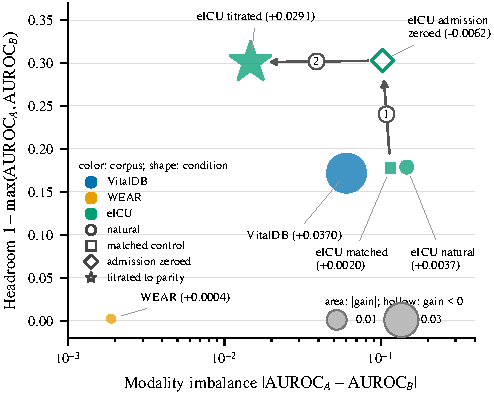
\includegraphics[width=\columnwidth]{fig06_fusion_map.pdf}
\caption{Fusion gain against modality imbalance and headroom (color: corpus; shape: condition; area: $|$gain$|$); numbered arrows trace the eICU titration.}
\label{fig:fusion}
\end{figure}

\subsection{Component Ablation and Membership-Inference Audit}
\label{sec:results:ablation}
Each component is removed in turn from the full system, three seeds paired
(case-level)
(Table~\ref{tab:ablation}, Fig.~\ref{fig:audit}(a)). Removing sparsification
($+0.0012$) or quantization ($+0.0001$, the narrowest interval in the study)
leaves accuracy unchanged and raises uplink fivefold and $1.6$-fold, so
compression is justified by traffic alone. Removing the edge tier costs
$-0.0058$ at three seeds and is resolved at the six pre-registered seeds,
$-0.0047$ $[-0.0088, -0.0006]$ on VitalDB and $-0.0052$
$[-0.0074, -0.0030]$ on WEAR; because the flat arm also changes the
aggregation schedule, this bounds the cost of the hierarchy rather than
claiming a benefit. Removing the privacy mechanism \emph{reduces} AUROC by
$0.0234$: two of three non-private seeds peak in the first round and then
degrade, whereas every private seed peaks between rounds six and nine, so
clipping and noise regularize a compact head over frozen features. The
loss-aware edge weighting of an earlier version (C6) adds nothing and is not
adopted.

\begin{table}[!t]
\centering
\caption{Component ablation on VitalDB (record-level mechanism, case-level partition, three seeds)}
\label{tab:ablation}
\small
\setlength{\tabcolsep}{4pt}
\begin{tabular}{llcr}
\toprule
Removed & AUROC & $\Delta$AUROC & MB \\
\midrule
--- (full)        & $0.8541$ & ---                  & $252$ \\
C1 hierarchy      & $0.8484$ & $-0.0058 \pm 0.0088$ & $50$ \\
C2 privacy        & $0.8307$ & $\mathbf{-0.0234 \pm 0.0205}$ & $252$ \\
C3 sparsification & $0.8553$ & $+0.0012 \pm 0.0083$ & $1260$ \\
C4 quantization   & $0.8543$ & $+0.0001 \pm 0.0006$ & $403$ \\
+C6 loss weighting & $0.8542$ & $+0.0001 \pm 0.0009$ & $252$ \\
\bottomrule
\end{tabular}
\tabnote{$\Delta$AUROC is paired against the full system; bold: the interval
excludes zero. MB: total uplink. C6 is an inclusion arm.}
\end{table}

\begin{figure*}[!t]
\centering
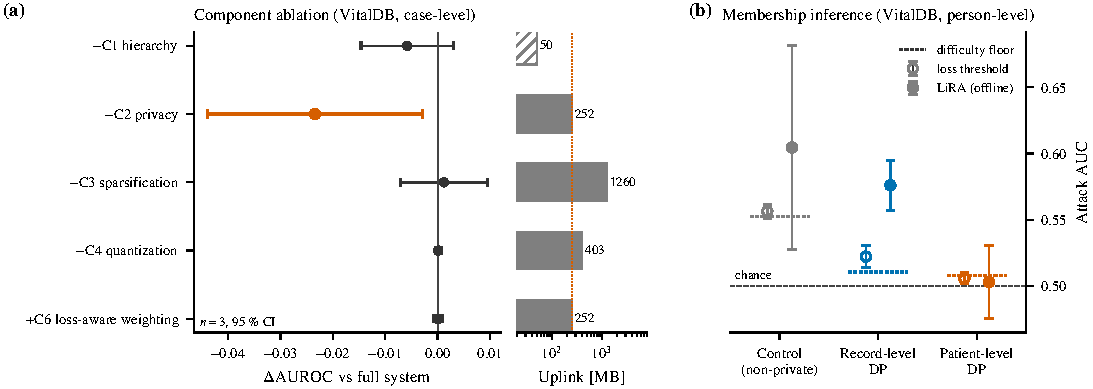
\includegraphics[width=\textwidth]{fig10_ablation_mia.pdf}
\caption{VitalDB: (a) component ablation, case-level ($\Delta$AUROC, $n = 3$, $95\,\%$ CI); (b) membership inference, person-level, against each difficulty floor (dotted).}
\label{fig:audit}
\end{figure*}

\emph{Audit.} Table~\ref{tab:mia} reports the leakage of three
configurations on the person-level partition. The positive control,
non-private training of the same head, shows that the audit detects
leakage: offline LiRA reaches $0.605$, $0.052$ above its difficulty floor and
$0.048$ above the loss threshold, and online LiRA with a global variance
reaches $0.597$ $[0.586, 0.609]$, entirely above the floor; at three seeds the
offline interval spans the floor. Record-level training remains detectably
above its floor under offline LiRA ($0.576$, margin $+0.065$), whereas
patient-level training does not ($0.503$, margin $-0.005$). The record-level
arm is not equivalent to the control: it lies below it under the loss
threshold ($0.522$ against $0.556$) and online LiRA with a global variance
($0.508$ against $0.597$), and the two were not compared statistically (three
control seeds against five). The attack that validates the control (online,
global variance) is thus not the one that separates the two units (offline).
Paired over five seeds on identical shadow
splits, the record-level arm exceeds the patient-level arm by $+0.073$
$[0.054, 0.092]$ ($p < 0.001$) for offline LiRA and by $+0.016$
$[0.010, 0.023]$ ($p = 0.002$) for the loss threshold, both surviving
correction for four attacks; the two online attacks resolve no difference.
The direction is as predicted, but the magnitude is smaller: the record-level
attack reaches $0.576$, not the predicted $0.7$. On the case-level partition,
where members were operations, no difference was resolved ($+0.029$
$[-0.038, +0.095]$ for offline LiRA). The audit covers VitalDB only and
bounds what these attacks achieve; it does not establish the absence of
leakage.

\begin{table}[!t]
\centering
\caption{Membership inference on VitalDB (person-level partition)}
\label{tab:mia}
\small
\setlength{\tabcolsep}{2.5pt}
\begin{tabular}{lccc}
\toprule
Configuration & Loss AUC & LiRA AUC & Floor \\
\midrule
Control (no DP) & $0.556$ {\scriptsize$[0.551, 0.561]$} & $0.605$ {\scriptsize$[0.528, 0.681]$} & $0.553$ \\
Record-level DP & $0.522$ {\scriptsize$[0.514, 0.531]$} & $0.576$ {\scriptsize$[0.557, 0.594]$} & $0.511$ \\
Patient-level DP & $0.506$ {\scriptsize$[0.502, 0.510]$} & $0.503$ {\scriptsize$[0.475, 0.531]$} & $0.508$ \\
\bottomrule
\end{tabular}
\tabnote{Mean attack AUC with $95\,\%$ interval over the target seeds (three
for the control, five otherwise); LiRA is the offline likelihood-ratio attack.
Floor: the AUC from per-patient difficulty alone, without the target model.}
\end{table}

\emph{Attribution.} Integrated gradients over $512$ test windows (case-level)
give the
$22$ missingness indicators $15.8\,\%$ of the prediction without privacy and
$21.6$--$21.7\,\%$ under either unit with frozen encoders, below their
$42\,\%$ share of inputs.

\subsection{Comparison with Prior Systems}
\label{sec:results:prior}
HED-FL \cite{ref3} and FL2DP \cite{ref9} were re-implemented and trained
through the same trainer, splits, frozen encoders, rounds and five seeds as
PP-HFM (Table~\ref{tab:prior}). HED-FL aggregates hierarchically without
privacy, uploads dense updates and samples $60\,\%$ of the clients per round;
FL2DP perturbs every coordinate with an exponential mechanism and shuffles the
updates, without a hierarchy. FL2DP was run on VitalDB only, because its
per-coordinate mechanism would take about two GPU days per seed on eICU.

\emph{Utility and traffic.} On VitalDB, PP-HFM exceeds FL2DP by $0.0123$
AUROC $[0.0064, 0.0181]$ and $0.025$ AUPRC $[0.015, 0.035]$, and HED-FL by
$0.030$ AUPRC $[0.005, 0.055]$; the AUROC difference from HED-FL, $0.0056$
$[-0.0018, +0.0131]$, is not resolved. HED-FL exceeds the non-private PP-HFM
reference by $0.0062$ AUROC $[0.0011, 0.0113]$.
On eICU, HED-FL is $3.17$ AUROC points $[1.56, 4.77]$ and $1.77$ AUPRC points
$[0.75, 2.78]$ above the private model and level with the non-private
reference ($+0.0008$, $p = 0.39$), so the gap is the price of the
patient-level guarantee measured in Section~\ref{sec:results:privacy}. PP-HFM
uploads $2.2$ times less than HED-FL on VitalDB, $2.4$ times less on eICU, and
$4.0$ times less than FL2DP.

\emph{Leakage.} On VitalDB, under the audit of
Section~\ref{sec:results:ablation}, on the same seeds and shadow splits, offline LiRA reaches $0.581$ against HED-FL
and $0.608$ against FL2DP, $0.078$ $[0.050, 0.106]$ and $0.105$
$[0.079, 0.130]$ above PP-HFM; the loss threshold gives $+0.047$ and
$+0.055$. Both baselines also have higher difficulty floors ($0.555$ and
$0.559$ against $0.508$), and their margins above them are $+0.026$ and
$+0.049$, against $-0.005$ for PP-HFM. The PP-HFM is the patient-level audit target, trained at $\varepsilon = 1.0$ with $\varepsilon_{\mathrm{conf}} = 0.5$ and one worst-client multiplier under the R\'enyi accountant, not the $\varepsilon = 0.9$ model whose AUROC and uplink are listed, so its leakage is measured at a slightly weaker budget than the headline. The comparison bounds what these attacks achieve and does not by itself establish the guarantee. FL2DP leaks more than HED-FL, which adds no noise at all.
Its candidate set is built from the private gradient value
(Eqs.~11--12 of \cite{ref9}), so the mechanism satisfies no finite
$\varepsilon$, and the audit finds that it does not reduce leakage either.

\begin{table}[!t]
\centering
\caption{PP-HFM against re-implemented prior systems (five seeds)}
\label{tab:prior}
\small
\setlength{\tabcolsep}{3pt}
\begin{tabular}{llcccc}
\toprule
& System & $\varepsilon$ & AUROC & MB & LiRA \\
\midrule
\multirow{3}{*}{\rotatebox{90}{\scriptsize VitalDB}}
& PP-HFM & $0.90$ & $\mathbf{0.8318}$ & $\mathbf{252}$ & $\mathbf{0.503}$ {\scriptsize$(-0.005)$} \\
& HED-FL & $\infty$ & $0.8262$ & $560$ & $0.581$ {\scriptsize$(+0.026)$} \\
& FL2DP & --- & $0.8195$ & $1008$ & $0.608$ {\scriptsize$(+0.049)$} \\
\midrule
\multirow{2}{*}{\rotatebox{90}{\scriptsize eICU}}
& PP-HFM & $0.90$ & $0.7936$ & $\mathbf{5235}$ & --- \\
& HED-FL & $\infty$ & $\mathbf{0.8252}$ & $12541$ & --- \\
\bottomrule
\end{tabular}
\tabnote{$\varepsilon$: patient-level training budget ($\delta = 10^{-5}$);
---: no finite bound. MB: total uplink. LiRA: offline attack AUC,
margin above the difficulty floor in parentheses; not run on eICU. The
PP-HFM LiRA entry is the patient-level audit target (Section~\ref{sec:method:mia}:
$\varepsilon = 1.0$, $\varepsilon_{\mathrm{conf}} = 0.5$, one worst-client
multiplier, R\'enyi accountant), not the $\varepsilon = 0.9$ model whose AUROC
and uplink are listed. eICU rows: source partition, on which the baselines
were run ($2.9\,\%$ of training persons at several hospitals,
Section~\ref{sec:method:privacy}). All AUROC
differences from PP-HFM are resolved except HED-FL on VitalDB.}
\end{table}

\section{Discussion}
\label{sec:discussion}

\subsection{What the Price of the Unit Depends On}
The central finding (RQ1, RQ2) is not that an individual-level guarantee has a cost,
which was expected, but that the cost has a regular shape. At one operating
point on person-level VitalDB it is $0.0170$ AUROC. Holding the per-step budget and the units per step
fixed, so that only the clipping geometry differs, it is indistinguishable
from zero at one record per individual and grows as $A(1-1/k)$, with a single
parameter that a fit on $k \le 4$ already determines. The patient-level model
stays flat while the record-level model improves, so a patient-level guarantee
becomes relatively more expensive, not cheaper, as more records are collected
per patient. Normalizing the clipping bound by the record count does not
recover the cost on eICU and could explain at most one eighth of it on VitalDB,
so the cost belongs mainly to the unit. Proposition~\ref{prop:scaling}
also points to what would: clipping around an estimate of each individual's
mean gradient, whose user-level rates improve with $k$ \cite{ref32}. The
external corpus reproduces the shape and the saturation but not the
magnitude: the relationship transfers in shape, its magnitude is
corpus-dependent, and outcome prevalence, client heterogeneity, contribution
counts and feature distributions are plausible contributors that the present
experiments do not isolate.

\subsection{Position Against Prior Art}
PP-HFM builds on user-level privacy \cite{ref11}
and parameter-efficient private fine-tuning \cite{ref12, ref13}; its
contribution is their composition inside a hierarchy, with a proof, and its
cost. Hierarchical systems
\cite{ref3, ref4, ref5} report savings without a guarantee, and private
systems \cite{ref9, ref10} leave the edge tier out of the accounting; PP-HFM
measures both on the same configuration and shows that the savings cost no
utility. The re-implemented baselines make this concrete
(RQ4; Section~\ref{sec:results:prior}). On eICU, HED-FL matches the non-private
reference, so its $3.2$-point lead over PP-HFM is the price of the
patient-level guarantee; on VitalDB, PP-HFM matches HED-FL in AUROC, exceeds
it in AUPRC, and leaks less under offline LiRA (margin $-0.005$ against $+0.026$). FL2DP adds noise yet leaks more than HED-FL, which adds none:
a perturbation without a finite $\varepsilon$ is not a weaker guarantee but
no guarantee, and only an audit can show what it protects. The parameter-efficient literature attributes
robustness at small $\varepsilon$ to the reduced privatized dimension; the
three-way decomposition attributes it to the initialization instead (RQ3), which
changes what a practitioner should optimize first. Several results are
negative and are reported with the control or the power that makes them
interpretable: the privatized subset produces no resolved accuracy effect once the
initialization is controlled, compression and loss-aware weighting produce no
resolved accuracy change, and count-normalized clipping does not recover the
cost of the unit on eICU. Within the evaluated configurations, they indicate
where engineering effort does not pay off in accuracy.

\subsection{Practical Implications}
Four recommendations follow. First, choose the unit explicitly and price it
in records per individual: where individuals contribute many records, a
record-level budget bounds the wrong quantity. Second, secure a legitimate
pretrained initialization before tuning anything else; under a tight budget
it is the largest effect measured here. Third, calibrate each client to its
own population (on eICU a single worst-case multiplier would impose $29.34$
on every hospital against a median need of $13.76$), and consider a minimum
cohort size, since the smallest hospitals set the cost. Fourth, use
compression and the edge tier, which cut traffic and energy at no measurable
cost in accuracy, and establish fusion per task. Before deployment, the
end-to-end conditions should hold, with disjoint pretrained encoders and
standardization constants fitted on a disjoint pool, as in the eICU end-to-end
configuration, and the simulated network and modeled energy figures should be
confirmed on physical hardware.

\subsection{Limitations}
\emph{Utility.} On eICU the cost of the guarantee is inconclusive against the
two-point target and exceeds it end to end (Section~\ref{sec:results:privacy});
on WEAR the record-level accuracy loss is inconclusive. \emph{Encoders and
unit.} VitalDB and WEAR utilities use oracle encoders unless stated and are
upper bounds; the disjoint encoders cost $1.57$ AUROC points and leave
differences between configurations unaffected. VitalDB analyses other than the
privacy cost, the cost of the unit, the baseline comparison and the audit are
case-level, covering persons with several operations only by group privacy;
WEAR is record-level; the eICU source partition is qualified in
Section~\ref{sec:method:analysis}; and the validation cohort selects
checkpoints without noise. \emph{Power.} The scaling grids and the recipe
sweep use three seeds, and resolving the eICU gaps of
Table~\ref{tab:kscaling} would need about twenty-five. The audit (sixteen
shadows, VitalDB only) cannot resolve a $0.1\,\%$ false-positive rate; it
bounds these attacks and does not establish the absence of leakage.
\emph{Baselines and simulation.} HED-FL and FL2DP are re-implemented from their
papers, with FL2DP and the baseline audits on VitalDB only, and round
latencies compare simulated topologies rather than a deployed system.
\emph{Fusion and theory.} A fusion gain is shown on VitalDB only, and the
$A(1-1/k)$ form is supported empirically, not proved.

\section{Conclusion}
\label{sec:conclusion}

This paper addressed a mismatch between what private hierarchical federated
learning guarantees and what clinical IoT requires: existing systems protect
individual records, whereas a clinical deployment must protect patients, each
of whom contributes many records. The proposed framework, PP-HFM, closes this
gap by construction. Each client sums a patient's gradients before clipping,
calibrates its noise to its own population, which parallel composition
permits for every patient held by one client, and accounts for every
release of the hierarchy, edge tier included. The guarantee was proved for the
training transcript; it holds end to end only when the encoders and
standardization constants are fitted on public data, which on the evaluated
corpora is the eICU configuration, and there for the $97.1\,\%$ of training
individuals treated at a single hospital.

The evaluation on three corpora supports four conclusions. First, the system
objectives are met on every corpus with two exceptions on eICU and one on
WEAR, where the record-level utility loss of $1.97$~pp is inconclusive
against the two-point target: the training
budget is at most $\varepsilon = 0.9$ ($1.0$ with the evaluated conformal
release), uplink traffic falls by $90.8$--$96.1\,\%$, modeled energy per
round by $72.3$--$79.6\,\%$, and the $95$th-percentile inference latency on
a workstation CPU is at most $2.3$~ms, but on eICU the utility loss exceeds
the two-point target end to end and is inconclusive against it with
training-fitted constants, and update delivery reaches
$99\,\%$ only from eight edges. Second, the patient-level guarantee is affordable: it costs no utility on
VitalDB, partitioned by person, and on eICU it costs $3.1$ AUROC points $[1.4, 4.8]$ ($3.9$ $[2.4, 5.4]$ end to
end), a cost set by the smallest hospitals. Third, on VitalDB and WEAR, robustness to a strict
budget is determined by the initialization, not by the size of the privatized
subset: pretrained initialization is worth $0.199$ AUROC at
$\varepsilon = 0.5$, whereas restricting noise to the head changes accuracy by
at most $0.006$ under privacy and is justified by communication alone. Fourth, the price of
an individual-level guarantee follows $A(1 - 1/k)$ in records per individual
and vanishes where the two units coincide, a scaling that holds out of sample
on the first corpus and in shape on the second. On VitalDB, a patient-level
audit with a positive control is consistent with the distinction: record-level
training remains detectably above its difficulty floor under offline LiRA,
whereas patient-level training does not; the audit bounds these attacks
without establishing the absence of leakage. The corpora carry different
evidence: eICU tests the guarantee end to end for individuals at one hospital, VitalDB tests it on the
training transcript, and WEAR, where each client is one participant,
evaluates the system at record level.

Several directions remain open. First, a third corpus is needed to determine
whether the ceiling of the cost curve is a constant of the guarantee or a
fraction of the precision attainable on a task. Second, the noise imposed by
the smallest clients could be reduced, for example by sampling patients across
the clients of an edge. Third, clipping around an estimate of each
individual's mean gradient, which the analysis indicates could recover the
cost of the unit, should be tested. Finally, the audit should be extended to eICU
and, with a larger shadow population, to low false-positive rates.

\section*{Data Availability}
VitalDB \cite{ref20} (\url{https://vitaldb.net}) and WEAR \cite{ref21} are
publicly available. The eICU Collaborative Research Database \cite{ref27} is
available through PhysioNet \cite{ref28} to credentialed users under a data
use agreement, so no patient-level records or arrays derived from them are
redistributed. All corpora are de-identified; this study is a secondary
analysis with no patient contact. Code and aggregate results will be released
upon publication.

% Acknowledgment removed at the authors' request (2026-11-04). IEEE policy asks
% for any AI-use disclosure and any funding statement in an Acknowledgment
% section; restore one here if either is needed.


\bibliographystyle{IEEEtran}
\bibliography{references}

\end{document}
